\documentclass[14pt,a4paper]{report}  %紙張設定
\usepackage{xeCJK}%中文字體模組
%\setCJKmainfont{標楷體} %設定中文字體
\setCJKmainfont{MoeStandardKai.ttf}
%\newfontfamily\sectionef{Times New Roman}%設定英文字體
\newfontfamily\sectionef{Nimbus Roman}
\usepackage{enumerate}
\usepackage{amsmath,amssymb}%數學公式、符號
\usepackage{amsfonts} %數學簍空的英文字
\usepackage{graphicx, subfigure}%圖形
\usepackage{fontawesome5} %引用icon
\usepackage{type1cm} %調整字體絕對大小
\usepackage{textpos} %設定文字絕對位置
\usepackage[top=2.5truecm,bottom=2.5truecm,
left=3truecm,right=2.5truecm]{geometry}
\usepackage{titlesec} %目錄標題設定模組
\usepackage{titletoc} %目錄內容設定模組
\usepackage{textcomp} %表格設定模組
\usepackage{multirow} %合併行
%\usepackage{multicol} %合併欄
\usepackage{CJK} %中文模組
\usepackage{CJKnumb} %中文數字模組
\usepackage{wallpaper} %浮水印
\usepackage{listings} %引用程式碼
\usepackage{hyperref} %引用url連結
\usepackage{setspace}
\usepackage{lscape}%設定橫式
\lstset{language=Python, %設定語言
		basicstyle=\fontsize{14pt}{4pt}\selectfont, %設定程式內文字體大小
		frame=lines,	%設定程式框架為線
}
%\usepackage{subcaption}%副圖標
\graphicspath{{./../images/}} %圖片預設讀取路徑
\usepackage{indentfirst} %設定開頭縮排模組
\renewcommand{\figurename}{\Large 圖 } %更改圖片標題名稱
\renewcommand{\tablename}{\Large 表 }
\renewcommand{\lstlistingname}{\Large 程式 } %設定程式標示名稱
\hoffset=-5mm %調整左右邊界
\voffset=-8mm %調整上下邊界
\setlength{\parindent}{3em}%設定首行行距縮排
\usepackage{appendix} %附錄
\usepackage{diagbox}%引用表格
\usepackage{multirow}%表格置中
%\usepackage{number line}
%=------------------更改標題內容----------------------=%
\titleformat{\chapter}[hang]{\center\sectionef\fontsize{20pt}{1pt}\bfseries}{\LARGE 第\CJKnumber{\thechapter}章}{1em}{}[]
\titleformat{\section}[hang]{\sectionef\fontsize{18pt}{2.5pt}\bfseries}{{\thesection}}{0.5em}{}[]
\titleformat{\subsection}[hang]{\sectionef\fontsize{16pt}{2.5pt}\bfseries}{{\thesubsection}}{1em}{}[]
%=------------------更改目錄內容-----------------------=%
\titlecontents{chapter}[11mm]{}{\sectionef\fontsize{18pt}{2.5pt}\bfseries\makebox[3.5em][l]
{第\CJKnumber{\thecontentslabel}章}}{}{\titlerule*[0.7pc]{.}\contentspage}
\titlecontents{section}[18mm]{}{\sectionef\LARGE\makebox[1.5em][l]
{\thecontentslabel}}{}{\titlerule*[0.7pc]{.}\contentspage}
\titlecontents{subsection}[4em]{}{\sectionef\Large\makebox[2.5em][l]{{\thecontentslabel}}}{}{\titlerule*[0.7pc]{.}\contentspage}
%=----------------------章節間距----------------------=%
\titlespacing*{\chapter} {0pt}{0pt}{18pt}
\titlespacing*{\section} {0pt}{12pt}{6pt}
\titlespacing*{\subsection} {0pt}{6pt}{6pt}
%=----------------------標題-------------------------=%             
\begin{document} %文件
\sectionef %設定英文字體啟用
\vspace{12em}
\begin{titlepage}%開頭
\begin{center}   %標題  
\makebox[1.5\width][s]
{\fontsize{24pt}{2.5pt}國立虎尾科技大學}\\[18pt]
\makebox[1.2\width][s]
{\fontsize{24pt}{2.5pt}機械設計工程暨精密機械工程科}\\[18pt]
\makebox[1.5\width][s]
{\fontsize{24pt}{2.5pt}專題製作報告}\\[18pt]
%設定文字盒子 [方框寬度的1.5倍寬][對其方式為文字平均分分布於方框中]\\距離下方18pt
\vspace{6em} %下移
\fontsize{30pt}{1em}\selectfont\textbf
{
\vspace{0.5em}
有限元素法在四足機器人設計上的
應用}\\

\vspace{1em}
\sectionef\fontsize{30pt}{1em}\selectfont\textbf
{
\vspace{0.5em}
Application of Finite Element Method
\vspace{0.5em}
to
 \vspace{0.5em} 
Quadruped Robot Design}
 \vspace{1em}
%=---------------------參與人員-----------------------=%             
\end{center}
\begin{flushleft}
\begin{LARGE}

\hspace{32mm}\makebox[5cm][s]
{指導教授:\quad 嚴\quad 家\quad 銘\quad 老\quad 師}\\[6pt]
\hspace{32mm}\makebox[5cm][s]
{\phantom{指導教授:\quad}李\quad 武\quad 鉦\quad 老\quad 師}\\[6pt]

\hspace{32mm}\makebox[5cm][s]
{班\qquad 級:\quad 四\quad 設\quad 三\quad 乙}\\[6pt]
\hspace{32mm}\makebox[5cm][s]
{學\qquad 生:\quad 楊\quad 子\quad 頡\quad(40923231)}
\\[6pt]
\hspace{32mm}\makebox[5cm][s]
{\hspace{36.5mm}楊\quad 建\quad 霖\quad(40923233)}\\[6pt]
\hspace{32mm}\makebox[5cm][s]
{\hspace{36.5mm}詹\quad 侑\quad 儒\quad(40923235)}\\[6pt]
\hspace{32mm}\makebox[5cm][s]
{\hspace{36.5mm}蔡\quad 宗\quad 瑋\quad(40923240)}\\[6pt]
%設定文字盒子[寬度為5cm][對其方式為文字平均分分布於方框中]空白距離{36.5mm}\空白1em
\end{LARGE}
\end{flushleft}
\vspace{4em}
\fontsize{18pt}{2pt}\selectfont\hspace{1em}\centerline{\makebox[\width][s]
{中華民國\hspace{3em} 
\hspace*{-1em}一~一~二\quad 年\quad 六\quad 月}}
\end{titlepage}
\newpage
%=---------------專題製作合可證明---------------------=%
 {\renewcommand\baselinestretch{1.4}\selectfont %設定以下行距
 {\begin{center}
    {\fontsize{20pt}{2.5pt} {國立虎尾科技大學}\\[8pt]{機械設計工程暨精密機械工程科}\\[8pt]{學生專題製作合格認可證明}\\
    \hspace*{\fill} \\ %似enter鍵換行
    \par}
     \end{center}}
    {\begin{textblock}{60}(1.85,0.8)
    \noindent \fontsize{15pt}{16pt}\selectfont 專題製作修習學生\enspace:\quad
    {\begin{minipage}[t]{10em}\underline{四設三乙\enspace 40923231\enspace 楊子頡}\\ \underline{四設三乙\enspace 40923233\enspace 楊建霖}\\ \underline{四設三乙\enspace 40923235\enspace 詹侑儒}\\ \underline{四設三乙\enspace 40923240\enspace 蔡宗瑋}\\ %下劃線符號指令
    \end{minipage}}
         \par} %結束指定行距
    {\renewcommand\baselinestretch{1.2}\selectfont %設定以下行距
    {\begin{textblock}{30}(1.8,4)
    \noindent \fontsize{16pt}{16pt}\selectfont 專題製作題目\enspace :有限元素法在四足機器人設計上的應用
    \hspace*{\fill} \\
    \hspace*{\fill} \\
    \noindent \fontsize{16pt}{16pt}\selectfont 經評量合格,特此證明
    \hspace*{\fill} \\
    \hspace*{\fill} \\
    \noindent \fontsize{16pt}{16pt} \makebox[6em][s]{評審委員}\enspace:\quad
    {\begin{minipage}[t]{6em} \underline{            }\\[16pt] \underline{            }\\[16pt] \underline{            }\\
    \end{minipage}}
    \end{textblock}}
    {\begin{textblock}{10}(1.8,9)
    {\begin{flushleft}
    \fontsize{16pt}{16pt}\selectfont \makebox[6em][s]{指導老師}\enspace:\quad \underline{            }\\[10pt]
    \fontsize{16pt}{16pt}\selectfont \makebox[6em][s]{系主任}\enspace:\quad \underline{            }\\
    \hspace*{\fill} \\
    \fontsize{16pt}{2.5pt}\selectfont \makebox[12em][s]{中華民國~一一二年}\hspace{2pt}
    \fontsize{16pt}{2.5pt}\selectfont\makebox[8em][s]{六月七日}
    \end{flushleft}}
    \end{textblock}}
    \end{textblock}}
     \par} %結束指定行距
    \thispagestyle{empty}
     \newpage

%=------------------------摘要-----------------------=%
\renewcommand{\baselinestretch}{1.5} %設定行距
\pagenumbering{roman} %設定頁數為羅馬數字
\clearpage  %設定頁數開始編譯
\sectionef
\addcontentsline{toc}{chapter}{摘~~~要} %將摘要加入目錄
\begin{center}
\LARGE\textbf{摘~~~要}\\
\end{center}
\begin{flushleft}
\fontsize{14pt}{20pt}\sectionef\hspace{12pt}\quad 本專題主要研究有限元素法(FEM),由於近代計算機快速的發展,數值計算、開發環境、生程式設計等,都有公司或個人創作者製作軟體進行分析、計算,藉由這些軟體我們將對四足機器人進行生成式設計並且觀察其受力情況。\\[14pt]
\fontsize{14pt}{20pt}\sectionef\hspace{12pt}\quad 以四足機器人為例,將結構以剛體狀況導入CoppeliaSim進行動作模擬後,求出最大反力分別帶入Ansys和Solid Edge,並在此轉換為柔性結構,進行有限元素(FEM)分析,評估各柔性結構下分析的應力、應變等受力情況,對其做生成式設計以簡化模組,在保有強度的同時減輕重量造成最少的能源浪費。並嘗試透過網路展示CoppeliaSim機器人運動情況,證明其設計可行性。\\[12pt]

\end{flushleft}
\begin{center}
\fontsize{14pt}{20pt}\selectfont 關鍵字:偏微分方程(PDE)、有限元素分析(PEM)、CoppeliaSim、Ansys、Solid Edge
\end{center}
\newpage

%=--------------------Abstract----------------------=%
\renewcommand{\baselinestretch}{1.5} %設定行距
\addcontentsline{toc}{chapter}{Abstract} %將摘要加入目錄
\begin{center}
\LARGE\textbf\sectionef{Abstract}\\
\begin{flushleft}
\fontsize{14pt}{16pt}\sectionef\hspace{12pt}\quad The main focus of this project is on the Finite Element Method (FEM). With the rapid development of modern computers, numerical calculations, development environments, and software programming, various companies or individual creators have developed software for analysis and calculations. With the help of these software programs, we will perform generative design on a quadruped robot and observe its structural integrity under various load conditions.\\[12pt]

\fontsize{14pt}{16pt}\sectionef\hspace{12pt}\quad Taking the quadruped robot as an example, we will import the structure as a rigid body into CoppeliaSim for motion simulation. After obtaining the maximum reaction forces, we will input them into Ansys and Solid Edge for further analysis. The rigid structure will then be converted into a flexible structure to perform Finite Element Method (FEM) analysis. We will evaluate the stress, strain, and other load conditions for each flexible structure to assess their performance. Through generative design, we aim to simplify the modules while maintaining their strength and minimizing energy waste caused by excessive weight. Additionally, we will attempt to showcase the motion of the robot in CoppeliaSim through online demonstrations to prove the feasibility of the design.\\
\end{flushleft}
\begin{center}
\fontsize{14pt}{16pt}\selectfont\sectionef Keywords: partial differential equation (PDE), finite element analysis (PEM), CoppeliaSim, Ansys, Solid Edge.
\end{center}

\newpage
%=------------------------謝辭----------------------=%
\addcontentsline{toc}{chapter}{誌~~~謝}
\centerline\LARGE\textbf{誌~~謝}\\
\begin{flushleft}
\fontsize{14pt}{2.5pt}\hspace{12pt}\quad 本專題能完成有著許多人員的幫忙,大四學長他們不吝嗇地將往年的製作經驗傳授給我們,讓我們在製作的時候少走了許多錯路,還總是貼心找出重點提醒我們可以加以描述。再來是我們的指導教授嚴家銘教授,他提供了多方面的資訊,拋出問題並給予建議,擬定了我們小組有限元素法研究和學習方向,開會也時常提出建議以及未來發展,得以順利解決遇到的技術問題,同時也給了相當程度的自由,讓小組得以有彈性去尋探索及摸索,而本專題組員也充分地付出了許多,讓專題研究能順利完成,從中獲益良多,特此感謝。
\end{flushleft}
\newpage
%=------------------------目錄----------------------=%
\renewcommand{\contentsname}{\centerline{\fontsize{18pt}{\baselineskip}\selectfont\textbf{目\quad 錄}}}
\tableofcontents  %目錄產生
\newpage
%=------------------圖表目錄產生----------------------=%
\renewcommand{\listfigurename}{\centerline{\fontsize{18pt}{\baselineskip}\selectfont\textbf{圖\quad 目\quad 錄 }}}
\newcommand{\loflabel}{圖} %定義\loflabel 文字為圖
\renewcommand{\numberline}[1]{\loflabel~\fontsize{14pt}{12pt}\selectfont #1\hspace*{0.5em}}
\listoffigures

\newpage

\renewcommand{\listtablename}{\centerline{\fontsize{18pt}{\baselineskip}\selectfont\textbf{表\quad 目\quad 錄 }}}
\newcommand{\lotlabel}{表} %定義\lotlabel 文字為表
\renewcommand{\numberline}[1]{\lotlabel~\fontsize{14pt}{12pt}\selectfont #1\hspace*{0.5em}}
\listoftables
%----------------------------------------%

\end{center}
%=-------------------------內容----------------------=%
\chapter{緒論}
\renewcommand{\baselinestretch}{10.0} %設定行距
\pagenumbering{arabic} %設定頁號阿拉伯數字
\setcounter{page}{1}  %設定頁數
\fontsize{14pt}{2.5pt}\sectionef

\section{研究動機與背景}
材料分析軟體的應用在機械領域愈來越廣泛,能夠將繪製零件進行分析,但卻鮮少人知道材料分析是怎麼進行的,背後所引用的代碼、原理的東西。本專題研究方向將由四足機器人作為設計主題,提供所需參數,將有限元素分析的公式套入並計算,對建模進行力學分析,用於設計優化,將透過本專題了解。(圖.\ref{fig.pong_gym})。\\
------------------------------------------------------
\begin{figure}[hbt!]
\begin{center}
\includegraphics[angle=90,width=10cm]{冰球機}
\caption{\Large 實體的冰球機}\label{fig.冰球機}
\end{center}
\end{figure}
-------------------------------------------------------
\begin{figure}[hbt!]
\begin{center}
\includegraphics[angle=90,width=10cm]{origin}
\caption{\Large 虛擬環境簡化後的冰球機}\label{fig.模擬冰球機}
\end{center}
\end{figure}
---------------------------------------------------------
\begin{figure}[hbt!]
\begin{center}
\includegraphics[height=8cm]{pong_gym}
\caption{\Large Gym的Pong game}\label{fig.pong_gym}
\end{center}
\end{figure}
--------------------------------------------------------------

\section{研究目的與方法}
本專題研究是以有限元素法有限元分析,Solid Edge繪出3D模型,並加入材質及各式力,測試不同部位所得出的物體模型的模擬分析,求出各個物理問題(應力、應變、變形等)。\\

以四足機械狗為模型,由solid edge建立3D模型,導入CoppeliaSim模擬環境,透過軟體的模擬功能,測試模型可行性,找出機器狗在運動時各部位的軌跡並找出反力為何。\\

接著利用Solid Edge分析,利用軟體中的有限元素法及各式方程式結合成的線性方程、進行代數求解、模擬,觀察、分析此模型在受力後的反應,篩選出適合的材料及形狀,透過此部分驗證材料的性質是否能夠負荷並擁有某些脆弱點,透過以上步驟可驗證實際運用上的此設計是否可行也可以讓設計者盡早發現錯誤並修正。\\
 -------------------------------------------------------------
\begin{figure}[hbt!]
\begin{center}
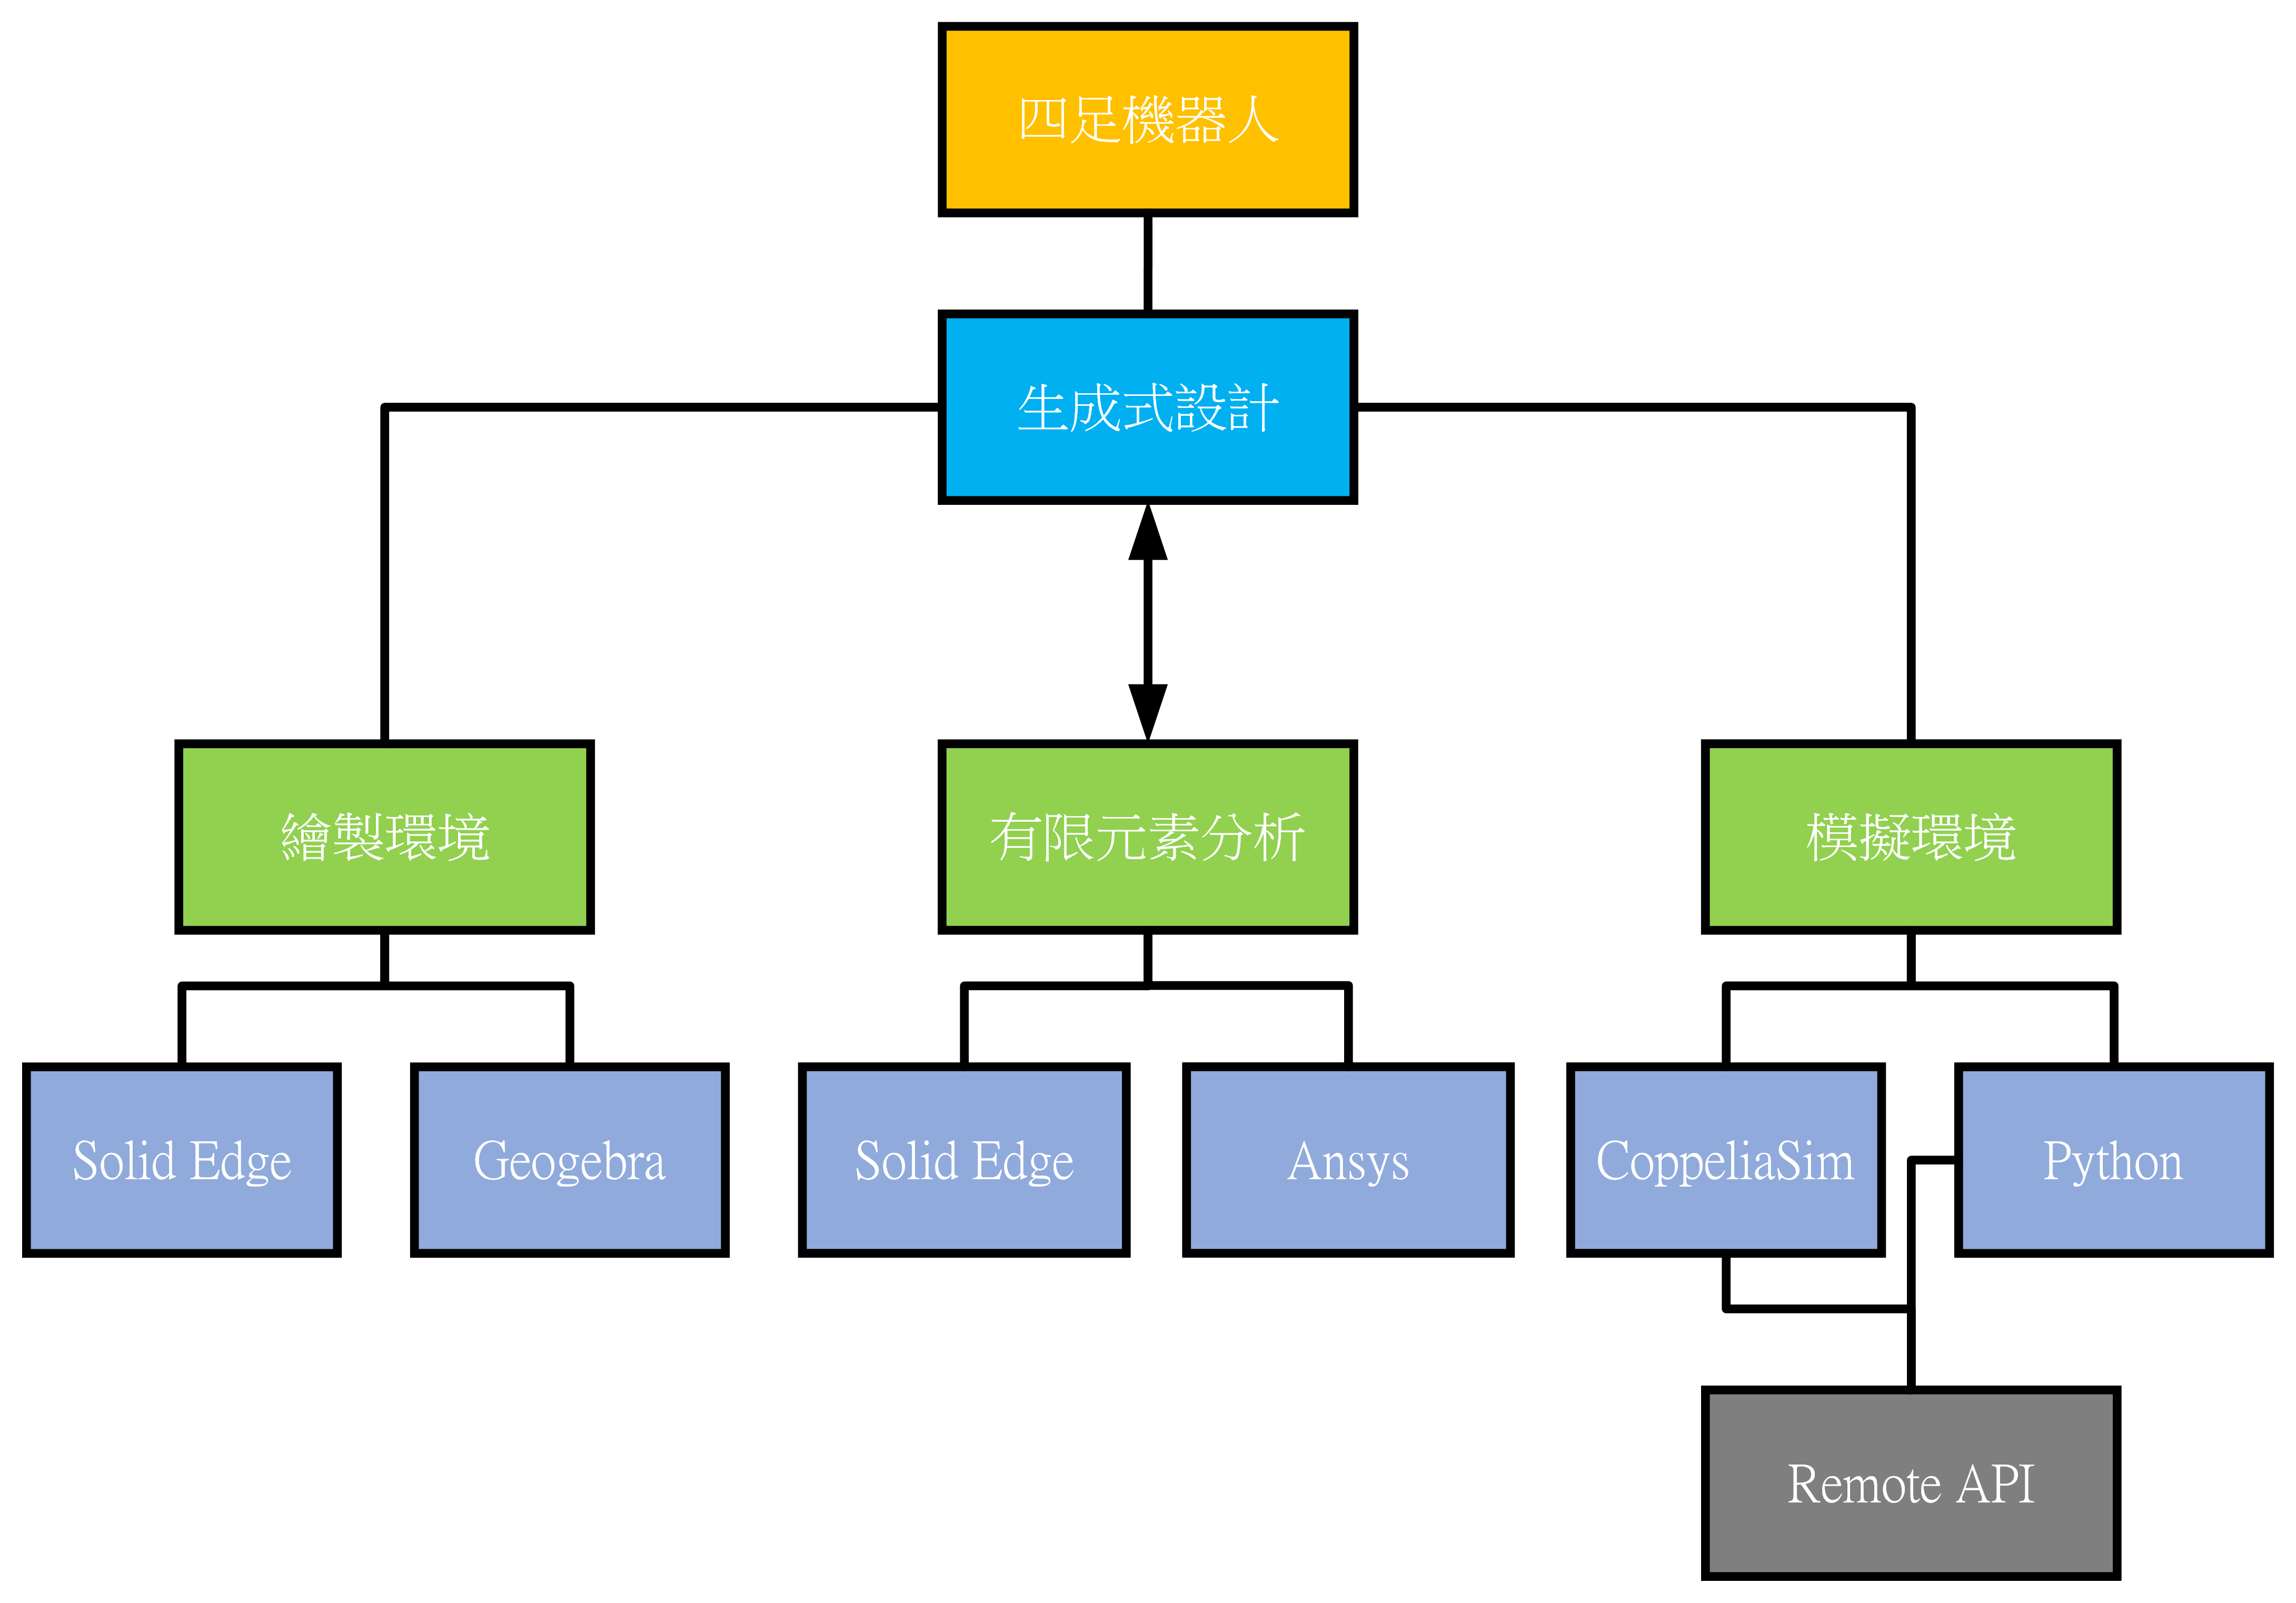
\includegraphics[width=15cm]{研究架構}
\caption{\Large 研究架構 }
\label{研究架構 }
\end{center}
\end{figure}
-------------------------------------------------------

\section{未來展望}

透過此研究可以求解出模型所受外力影響的數值變化,若之後可以對軟體輸入參數及設計因子,則軟體可以在所設定的範圍中透過計算產生設計者所需的模型並且,不再只局限於設計者的想像力,或是透過手機的日漸進步的激光雷達掃描系統,可以讓許多用戶都可以輕易地使用分析功能。\\

\section{分析說明}

模型進行運動分析後,透過求出的反力做為設計參數,帶入到至應力分析軟體中,並帶入合適的材料,通過預設的安全係數為最終目標。\\

\renewcommand{\baselinestretch}{0.5} %設定行距

\chapter{有限元素法}

\begin{figure}[hbt!]
\begin{center}
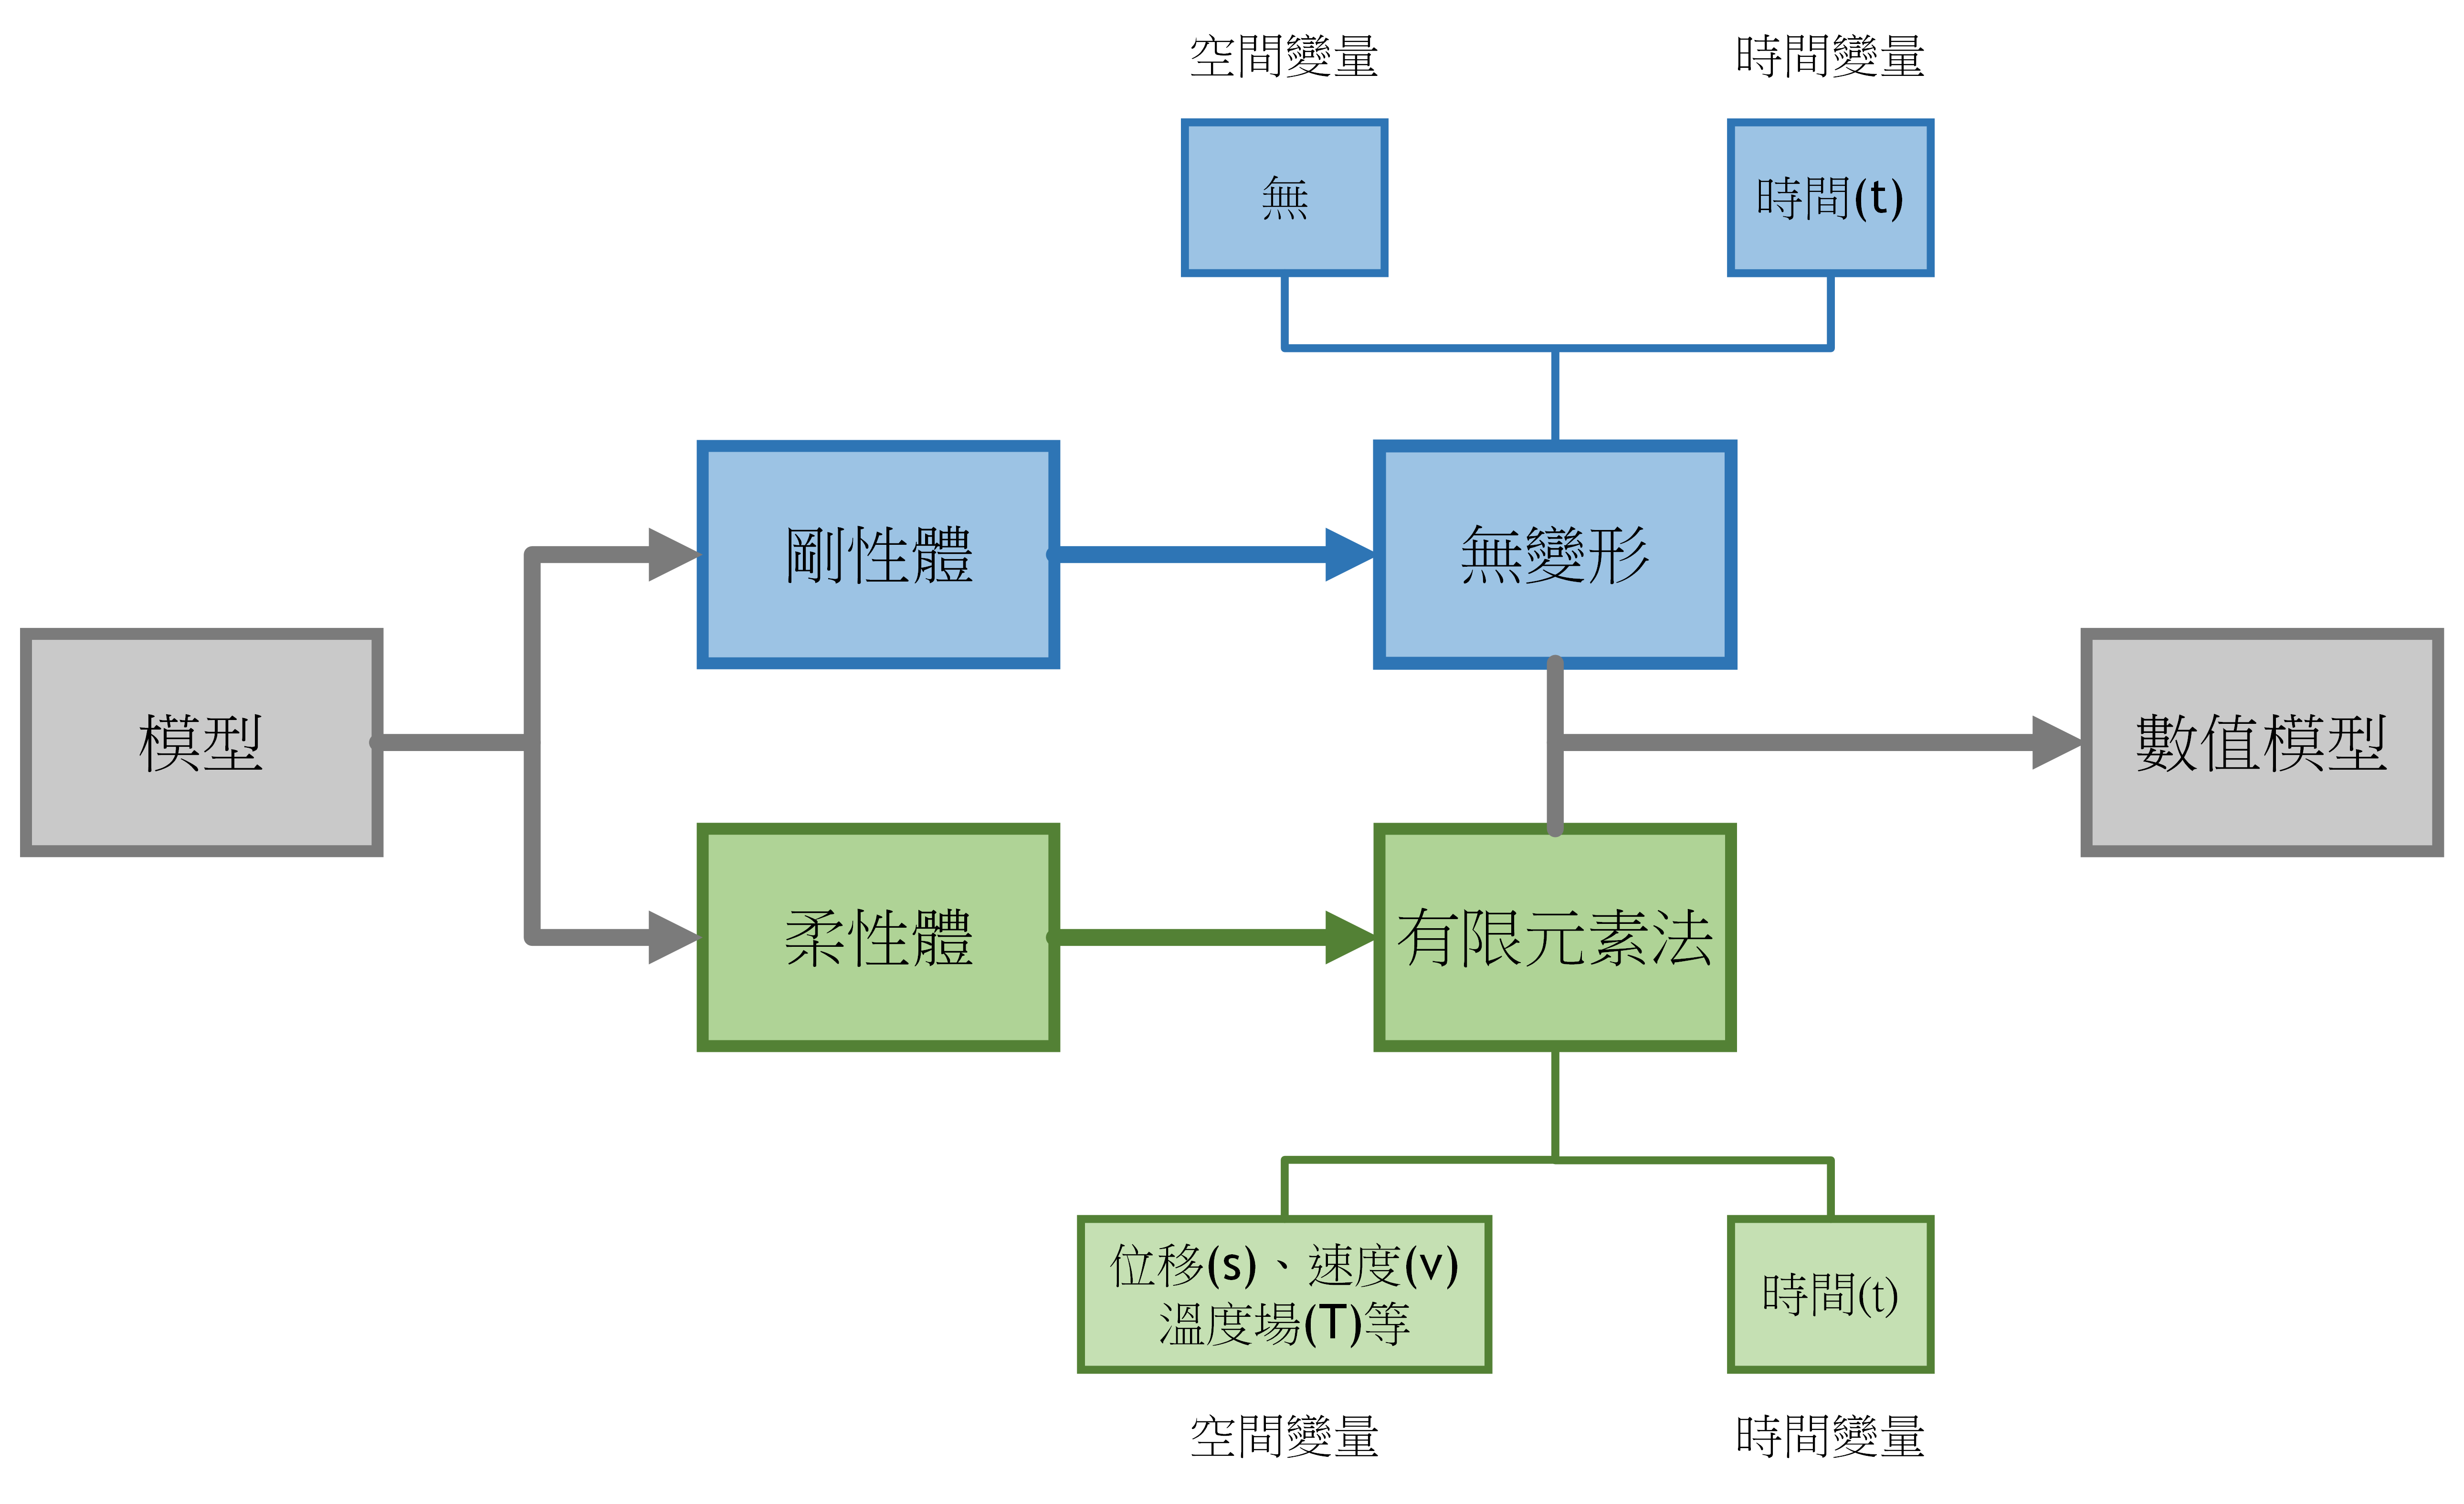
\includegraphics[width=15cm]{有限元素法}
\caption{\Large 有限元素法介紹}\label{有限元素法}
\end{center}
\end{figure}
時間及空間等問題常用偏微分方程(PDE)做數值求解,將根據不同的模型進行弱化、離散化等求解,此動作稱為有限元素法(FEM)。\\

通過在模型上簡化連續變量的複雜性來實現近似求解,常用於複雜的工程結構或物理系統的行為。\\

正因為剛體是理想狀態,現實中機器狗為柔性體,會因為受力情況的不同而產生多種變量,才需要利用偏微分方程對物體進行計算,此動作稱為有限元素法。\\

有對複雜模型進行分析及簡化的功能,所以在近代被廣泛的使用,在機械、建築等領域都可以看到其身影。\\

\newpage
%---------------------第二章/基本概念及假設假定-------------------------%
\section{基本概念}


\begin{figure}[hbt!]
\begin{center}
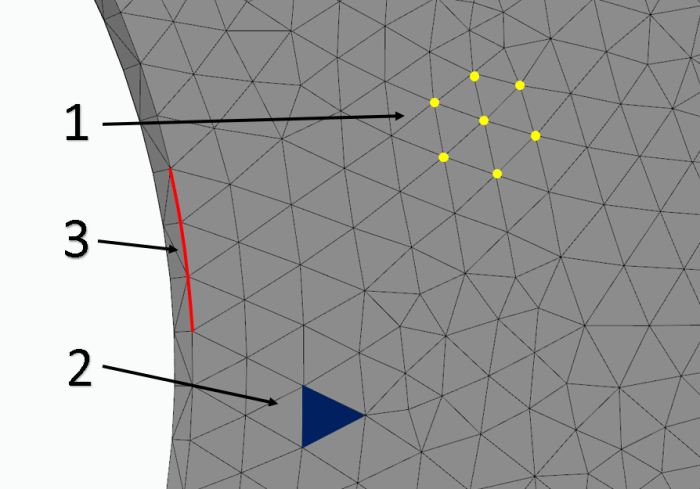
\includegraphics[width=8cm]{有限元素法介紹}
\caption{\Large 基本概念}
\label{有限元素法介紹}
\end{center}
\end{figure}

\begin{enumerate}
\item 節點:每個元素的角落或中心點,用於連接元素之間的邊界條件和解決方程,如(圖 \ref{有限元素法介紹})上1指示。
\item 元素:通常由三角形或者四邊形等形成的區域結構,如(圖 \ref{有限元素法介紹})上2所示。
\item 邊界條件:存在於物理系統邊界如(圖 \ref{有限元素法介紹})上3所示的約束及負荷力,模擬實際情況下的條件約束和外界影響。
\item 自由度: 節點上變量的個數,例如位移的節點自由度為3,表示單個節點擁有三個坐標方向的位移,又例如熱分析時節點自由度為1,表示某個節點處的溫度。
\item 網格:由數個元素經由節點連接所組成,表示在需分析的區域上。
\item 變形:邊界條件的影響下的形變,為分析後計算每個元素的變形及變形之間的相互影響,用以預測整得系統變化。
\item 離散化:將物理系統或結構等連續變量通過計算轉換為數格元素的過程,目的在於減化連續變量的複雜性,便於處理及分析。關於公式及步驟會因為模型或求解類型不同而有不一樣的計算方式。
\item 材料特性:物理系統(模型)的材料性質,不同的材料有著不一樣的參數(彈性模數、蒲松比、極限強度、降伏強度等)。\\
\end{enumerate}

\subsection{邊界條件}
分為兩種邊界條件,位移或施加力條件。

\begin{enumerate}
\item 位移邊界條件:規定了結構或邊界上的位移及變形的特定值或關係。

\begin{itemize}
\item 固定邊界條件:也稱為約束邊界條件,令特定的某些節點或自由度的位移為零,使其無法發生位移。
\item 位移約束:指定特定節點或自由度的位移值, 可以是定值或隨時間變化的函數。
\item 斜率約束:規定特定節點的自由度的位移斜率(導數),用於描述特定邊界上的傾斜或旋轉。
\end{itemize}

\item 力邊界條件:規定了結構或邊界上施加的外部力或力的分布。

\begin{itemize}
\item 負荷:施加在結構上的集中力或分布力,可以是靜態或動態負荷。
\item 壓力:施加在邊界上的或表面力,可以是均勻或非均勻的。
\item 動力學條件:施加在結構上的動態加載。\\
\end{itemize}
\end{enumerate}

\subsection{網格劃分基本原則}

\begin{enumerate}
\item 網格數量:將決定計算精度及規模大小,一般狀況中,網格數量增加計算精度也會跟著提升,但伴隨而來的是更大的計算量,所以在制定網格大小時應權衡兩個因素。
\item 網格疏密:在某些變化梯度較大的部位(應力集中處),需要大密集的網格,密集網格將更好反映數據變化,反之變化梯度較小的部位則用較稀疏的網格,而不同單元之間的連接則採用特殊的過度單元或多點約束等方法連接,才能更好的分配資源,兼顧計算量和計算精度。
\item 網格質量:網格形狀的合理性,質量的好壞將直接影響計算精度,質量較差的除了造成局部的計算精度偏差甚至會直接終止計算,因此在重要部位時應該確保其擁有高品質的表現,如果網格都是由等邊三角形、正方形、正四面體、立方六面體等組成,則求解精度可以非常接近實際值,但這種只存在於理想狀態下,實際運用卻很難做到。
\end{enumerate}

\begin{itemize}
\item 元素質量評價指標
\end{itemize}
\begin{enumerate}
\item 單元的邊長比、面積比及體積比,理想的邊長比為1,以正三角形、正四面體、正六面體為參考基準。
\item 扭曲度:單元內部扭轉及面外的翹曲程度。
\item 疏密過渡:應力梯度方向和橫向過渡情況,應力集中部分應較為密集,則反之。
\item 節點、元素排部:合理的節點及元素有助於帶入方程式計算,可以提高求解效率,但須注意消除重複的節點及元素。
\end{enumerate}

下列為網格疏密不同造成的分析差\

\begin{figure}[htbp]
  \centering
  \begin{minipage}{0.45\textwidth}
    \centering
    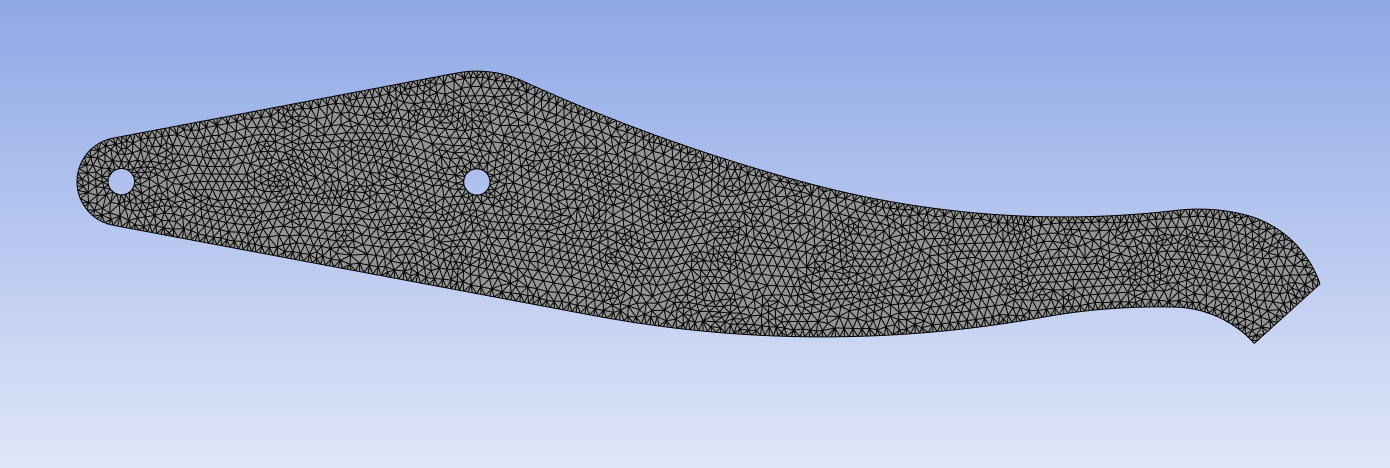
\includegraphics[width=\textwidth]{網格1mm-1}
    \caption{較密網格}
    \label{網格1mm-1}
  \end{minipage}
  \hfill
  \begin{minipage}{0.45\textwidth}
    \centering
    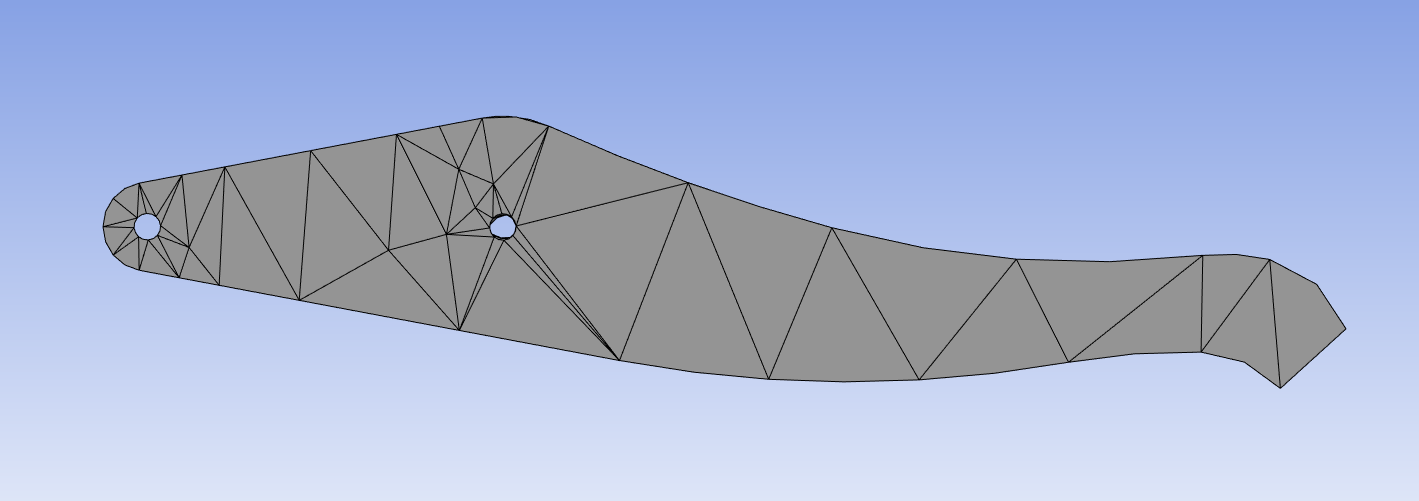
\includegraphics[width=\textwidth]{網格50mm-1}
    \caption{較粗網格}
    \label{網格1mm-2}
  \end{minipage}
  
  \begin{minipage}{0.45\textwidth}
    \centering
    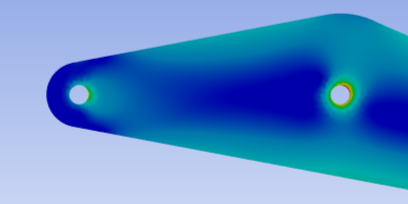
\includegraphics[width=\textwidth]{網格1mm-2}
    \caption{較密網格所得應力雲圖}
    \label{網格50mm-1}
  \end{minipage}
  \hfill
  \begin{minipage}{0.45\textwidth}
    \centering
    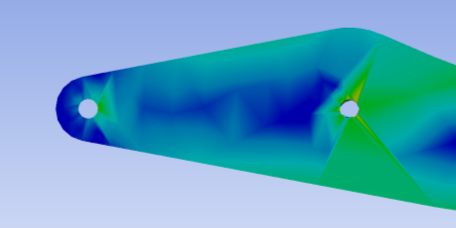
\includegraphics[width=\textwidth]{網格50mm-2}
    \caption{較粗網格所得應力雲圖}
    \label{網格50mm-2}
  \end{minipage}
\end{figure}
\newpage

%--------------------------第二章/有限元計算公式--------------------------%
\section{計算及公式介紹}
此章節主要介紹常見的結構力學的有限元計算公式及方法順序,了解到平時由電腦計算的有限元素法及代數方程式,觀察固體結構上變形及應力是如何進行分析計算以及選用原因。\\

\subsection{變形分析}

在有限元素分析中,通常使用拉格朗日公式,透過觀察材料的平移或旋轉來建立力學方程。
在材料上設置隨意點(X),觀察點(X)隨時間(t)變化後的材料位移矢量u(X,t),轉換為空間坐標系x=X+u即可以得到一個拉格朗日公式,只要材料為柔性體就會產生局部變化,此現象稱為應變或伸長,下列將透過多種方式來描述材料變形過程。\\

\begin{itemize}
\item 變形梯度
\end{itemize}

變形梯度F定義為
$$\mathbf{F}=\frac{\partial \mathbf{x}}{\partial \mathbf{X}}=\mathbf{I}+\frac{\partial \mathbf{u}}{\partial \mathbf{X}}$$\

其中, $\mathbf{I}$ 是等同張量, 展開為矩陣形式為:\

$$\mathbf{F}=\left[\begin{array}{lll}
\frac{\partial x}{\partial X} & \frac{\partial x}{\partial Y} & \frac{\partial x}{\partial Z} \\
\frac{\partial y}{\partial X} & \frac{\partial y}{\partial Y} & \frac{\partial y}{\partial Z} \\
\frac{\partial z}{\partial X} & \frac{\partial z}{\partial Y} & \frac{\partial z}{\partial Z}
\end{array}\right]=\left[\begin{array}{ccc}
1+\frac{\partial u}{\partial X} & \frac{\partial u}{\partial Y} & \frac{\partial u}{\partial Z} \\
\frac{\partial v}{\partial X} & 1+\frac{\partial v}{\partial Y} & \frac{\partial v}{\partial Z} \\
\frac{\partial w}{\partial X} & \frac{\partial w}{\partial Y} & 1+\frac{\partial w}{\partial Z}
\end{array}\right]$$
\\

上述矩陣包含材料局部旋轉和變形的完整解釋,其中還顯示許多訊息,例如:\

由於dx=FdX,未變形體dX中小線段是如何旋轉並拉伸,成為變形體dX中的線段,我們將F張量看做一個矩陣,第一列提供線段最開始沿X方向的大小和方向等信息。從數學角度來看,F是從X改變到x的Jacobi矩陣,因此它的行列式J=det(F)為局部體積比例因子,而不可壓縮材料$J=1$。\\

極分解定理表明,任何二階張量都可以分解為純轉動和對稱張量的乘積,利用這一定理將剛體轉動與變形分開:\
$$F=R U$$

這可以解釋為先發生變形(伸長張量$U$),再進行剛性旋轉(旋轉矩陣$R$)。如此一來,如果沒有旋轉,右伸長張量則為變形梯度,因此U的解釋與F類似。\\

同樣也可以將變形梯度分解為\
$$F=V R$$

此過程中,會先發生剛體轉動,然後轉動的體發生變形,變形透過左伸長張量V描述。\\

這兩個伸長張量$U$、$V$通過純轉動進行關聯,例如$\mathbf{V}=\mathbf{F R}^T=\mathbf{R} \mathbf{U} \mathbf{R}^T$。事實上此處旋轉矩陣的轉置也是自身的逆 $\left(\mathbf{R}^T \mathbf{R}=\mathbf{R R}^T=\mathbf{I}\right)$ 。\\

在實際操作中,極分解的計算成本通常較高,因此,人們會盡量避免這種類型的計算。但在理論思考方面,這個概念非常有用。我們可以在不確定旋轉矩陣的情況下,計算與旋轉無關的變形測量:\
$$\mathbf{F}^T \mathbf{F}=(\mathbf{R U})^T \mathbf{R} \mathbf{U}=\mathbf{U}^T \mathbf{R}^T \mathbf{R} \mathbf{U}=\mathbf{U}^T \mathbf{U}=\mathbf{U}^2=\mathbf{C}$$

張量C稱為右Cauchy-Green變形張量。\\

這個張量經常用於描述超彈性材料的本構特性等,僅由U張量構成,因此用於描述材料在旋轉“之前”的變形。\\

由此可知\
$$\mathbf{F} \mathbf{F}^T=\mathbf{V R}(\mathbf{V R})^T=\mathbf{V R R}^T \mathbf{V}^T=\mathbf{V} \mathbf{V}^T=\mathbf{V}^2=\mathbf{B}$$

張量B稱為左Cauchy-Green變形張量。\\

B和C都與旋轉無關,但它們描述的是兩個不同坐標系中的變形。\

張量C是描述材料坐標系中變形的材料張量,B是描述空間坐標系中變形的空間張量。\\

\begin{itemize}
\item 伸長率
\end{itemize}
從非正式意義上來說,伸長率可定義為當前長度與原始長度之比\
$$\lambda=\frac{L}{L_0}$$

因此在末變形狀態下,伸長率為1。一般情況下,人們更傾向於使用張量U和C的特徵值。U的三個特徵值$\left(\lambda_1\right)$、$\left(\lambda_2\right.$ 和 $\left.\lambda_3\right)$稱為主伸長率,其對應的特徵矢量在材料坐標系中給出三個正交方向。如果我們研究一個小立方體(正方體),其中三條邊沿著這三個方向,則它將會發生變化成為長方體,但所有邊仍保持直角相交。邊長變化由主伸長率表示。\
如此一來體積變化可以寫為主伸長率的乘積:\
$$\frac{V}{V_0}=\lambda_1 \lambda_2 \lambda_3$$\

張量C的計算更加簡單,它的主方向與U相同,但特徵值為$\lambda_1^2$、$\lambda_2^2$和$\lambda_3^2$。因此通常使用C而非U來計算主伸長率。\\

對於未變形材料(剛體)C=I。解釋了為甚麼在實際中人們主要使用C來描述較大伸縮性的材料。\\

左柯西-格林變形張量B也具有主伸長率作為特徵值。但由于V描述剛體轉動之後的伸長率,因此主方向依照空間方向來確定。\\

\begin{itemize}
\item 應變張量
\end{itemize}

要得到基于零的變形測量值,需要從C中減去等同張量,從而得到格林-拉格朗日應變張量E定義為\
$$\mathbf{E}=\frac{1}{2}(\mathbf{C}-\mathbf{I})$$

該張量也描述材料在發生任何轉動之前產生的變形,但在未變形狀態下的所有分項均為零,其分項可以寫為\
$$E_{i j}=\frac{1}{2}\left(\frac{\partial u_i}{\partial X_j}+\frac{\partial u_j}{\partial X_i}+\frac{\partial u_k}{\partial X_i} \frac{\partial u_k}{\partial X_j}\right)$$\

其中假設對重複指標求和。\\

格林-拉格朗日應編張量的對角元素如下\
$$E_{X X}=\frac{\partial u}{\partial X}+\frac{1}{2}\left(\left(\frac{\partial u}{\partial X}\right)^2+\left(\frac{\partial v}{\partial X}\right)^2+\left(\frac{\partial w}{\partial X}\right)^2\right)$$\

非對角元素的示例為\
$$E_{X Y}=\frac{1}{2}\left(\frac{\partial u}{\partial Y}+\frac{\partial v}{\partial X}+\frac{\partial u}{\partial X} \frac{\partial u}{\partial Y}+\frac{\partial v}{\partial X} \frac{\partial v}{\partial Y}+\frac{\partial w}{\partial X} \frac{\partial w}{\partial Y}\right)$$\

當應變和剛體轉動幅度都很小時,格林-拉格朗日應編張量中的二次項可以忽略不計,由此可得到工程應變張量\

$$\varepsilon_{i j}=\frac{1}{2}\left(\frac{\partial u_i}{\partial X_j}+\frac{\partial u_j}{\partial X_i}\right)$$\

其分量如下\
$$\varepsilon_{X X}=\frac{\partial u}{\partial X}$$\

和\
$$\varepsilon_{X Y}=\frac{1}{2}\left(\frac{\partial u}{\partial Y}+\frac{\partial v}{\partial X}\right)$$\

該應變張量的對角項稱為法向應變或正應變,用於描述沿每個坐標軸的延伸。非對角項是應變張量的剪切分量,用於描述線段之間夾角的變化。這裡的術語很容易被混淆,因為在工程領域,由於$\gamma_{i j}$直接測量角度的變化(以弧度表示),所以人們習慣使用“剪切應變”一詞來描述物理量$\gamma_{i j}=2 \varepsilon_{i j}=$
剪切應變產生等體積變形;即變形不引起體積改變。對於小應變相對體積變化通過正應變之和求得:\
$$\frac{\Delta V}{V}=\varepsilon_{x x}+\varepsilon_{y y}+\varepsilon_{z z}=\operatorname{trace}(\varepsilon)$$

\begin{itemize}
\item 真實應變
\end{itemize}

有時,我們會使用真實應變 這個術語。在真實應變的單軸定義中,應變增量定義為\
$$d \varepsilon=\frac{d L}{L}$$\

真實應變的定義基於當前長度,因此在積分後可以得到\
$$\varepsilon=\ln \left(\frac{L}{L_0}\right)=\ln (\lambda)$$\

這就是真實應變也稱為對數應變的原因。\\

\begin{itemize}
\item 應變協調性
\end{itemize}

由於應變張量由位移的導數構成,因此並非所有應變場均適用。位移矢量只有三個分量,這意味著,除非各個應變分量都滿足特定的協調性標準,否則它們的積分無法給出唯一的一組位移。工程應變必須滿足以下方程:\
$$\frac{\partial^2 \varepsilon_{i j}}{\partial X_k \partial X_l}+\frac{\partial^2 \varepsilon_{k l}}{\partial X_i \partial X_j}-\frac{\partial^2 \varepsilon_{i k}}{\partial X_j \partial X_l}-\frac{\partial^2 \varepsilon_{j l}}{\partial X_i \partial X_k}=0$$\

由於應變張量的對稱性,這81 個方程中只有6 個是非平凡方程。如下所示:\
$$
\begin{aligned}
\frac{\partial^2 \varepsilon_{x x}}{\partial y \partial z} & =\frac{\partial}{\partial x}\left(-\frac{\partial \varepsilon_{y z}}{\partial x}+\frac{\partial \varepsilon_{z x}}{\partial y}+\frac{\partial \varepsilon_{x y}}{\partial z}\right) \\
\frac{\partial^2 \varepsilon_{y y}}{\partial z \partial x} & =\frac{\partial}{\partial y}\left(-\frac{\partial \varepsilon_{z x}}{\partial y}+\frac{\partial \varepsilon_{x y}}{\partial z}+\frac{\partial \varepsilon_{y z}}{\partial x}\right) \\
\frac{\partial^2 \varepsilon_{z z}}{\partial x \partial y} & =\frac{\partial}{\partial z}\left(-\frac{\partial \varepsilon_{x y}}{\partial z}+\frac{\partial \varepsilon_{y z}}{\partial x}+\frac{\partial \varepsilon_{z x}}{\partial y}\right) \\
2 \frac{\partial^2 \varepsilon_{x y}}{\partial x \partial y} & =\frac{\partial^2 \varepsilon_{x x}}{\partial y^2}+\frac{\partial^2 \varepsilon_{y y}}{\partial x^2} \\
2 \frac{\partial^2 \varepsilon_{y z}}{\partial y \partial z} & =\frac{\partial^2 \varepsilon_{y y}}{\partial z^2}+\frac{\partial^2 \varepsilon_{z z}}{\partial y^2} \\
2 \frac{\partial^2 \varepsilon_{z x}}{\partial z \partial x} & =\frac{\partial^2 \varepsilon_{z z}}{\partial x^2}+\frac{\partial^2 \varepsilon_{x x}}{\partial z^2}
\end{aligned}
$$\

\subsection{應力方程}

\begin{itemize}
\item 動量平衡
\end{itemize}

作用在變形區域上的表面力可以表示為\
$$d \mathbf{F}_s=\mathbf{t}_n d a=\mathbf{T}_N d A$$\

其中$\mathbf{t}_{\mathrm{n}}$稱為牽引力,而 $\mathbf{T} \mathrm{N}$通常稱為標稱牽引力,原因是它將實際變形狀態下的作用力與未變形區域關聯起來。\\

此外,我們還可以基於法矢將牽引分量寫為以下線性展開式:\
$$T_i=P_{i J} N_J$$\

在此處和下文中,假設對重複指標求和。空間分量和材料分量分別使用小寫和大寫字母。這種表示有時稱為柯西定律或柯西公式,僅適用於$P_{i J}$為特定二階張量的分量的情況。對於任意未變形的材料體積$V_0$ ',動量守恆可以用以下積分形式表示:\
$$\frac{d}{d t} \int_{V_0} \rho_0 \mathbf{v} d V=\int_{V_0} \mathbf{f}_V d V+\int_{\partial V_0} \mathbf{T} d A$$\

其中$\mathbf{f}_V$ 表示體積力\\

速度場根據位移場 $\mathbf{u}$計算為\

$$\mathbf{v}=\frac{\partial \mathbf{u}}{\partial t}(\mathbf{X}, t)$$

根據散度定理,使用柯西公式可以將表面積分轉換為體積積分:\
$$\int_{\partial V_0} T_i d A=\int_{\partial V_0} P_{i J} N_J d A=\int_{V_0} \frac{\partial P_{i J}}{\partial X_J} d V$$\

因此可以得到動量平衡方程的微分形式如下所示:\
$$\rho_0 \frac{\partial^2 u_i}{\partial t^2}=f_{V, i}+\frac{\partial P_{i, J}}{\partial X_J}$$\

或者使用張量符號:\
$$\rho_0 \frac{\partial^2 \mathbf{u}}{\partial t^2}=\mathbf{f}_V+\nabla_X \cdot \mathbf{P}^{\mathbf{T}}$$\

張量P稱為第一類Piola-Kirchhoff應力張量,它將空間方向的作用力與原始未變形構型中的區域關聯起來。量指標涉及不同的構型。有時這種數學對象稱為兩點張量。\\

在實際的變形構型中,可以對牽引矢量$\mathrm{t}_{\mathrm{n}}$和材料體積應用類似的方法,可用下式表示:\
$$\mathbf{t}_n=\sigma_{i j} n_j \mathbf{e}_i$$\

張量$\sigma$ 稱為柯西應力張量或真實應力張量,原因是它表示與實際變形區域相關的實際構型中的力。由其空間分量表示。\\

由於柯西應力張量和第一類Piola-Kirchhoff 應力張量對同一個表面力有著不同的表示\
$$\mathbf{P N} d A=\sigma \mathbf{n} d a$$\

要確定這兩種應力測量方式之間的關係,我們可以使用Nanson公式 計算變形引起的面積變化,表示為\
$$\mathbf{n} d a=J \mathbf{F}^{-T} \mathbf{N} d A$$\

其中,F為變形梯度張量,由此可得\
$$J=\operatorname{det}(\mathbf{F})=d V / d V_0$$\

體積因子J可以給出變形引起的體積變化。因此,應力張量可通過下式與之關聯\
$$\mathbf{P}=J \sigma \mathbf{F}^{-T}$$\

通過引入一個稱為基爾霍夫應力張量(定義為$\tau=J \sigma$ )的張量,可以進一步簡化這個公式及類似公式。基爾霍夫應力張量是一個幾乎沒有實際用途的物理量,但卻具有理論上的便利性。\\

\begin{itemize}
\item 機械能平衡
\end{itemize}

將動量方程的微分形式乘以速度矢量,並基於材料對其進行積分,可以得到以下方程:\
$$\frac{d}{d t} \int_V \frac{1}{2} \rho v^2 d V+\int_V \sigma: \mathbf{L} d V=\int_V \mathbf{f}_v \cdot \mathbf{v} d V+\int_{\partial V} \mathbf{t}_n \cdot \mathbf{v} d A$$\

這個方程給出了機械能平衡的積分形式,也稱為冪定理。速度的空間梯度為$\mathbf{L}=\nabla_x \mathbf{V}$,其中的運算符表示對兩個指標求和\
$$\int_V \sigma: \mathbf{L} d V=\int_{V_0} \mathbf{P}: \dot{\mathbf{F}} d V_0$$\

變形分析頁面對速度梯度的特性進行了詳細論述。\\

方程右側的兩個積分項分別表示體積力和表面力的功率輸入,它們分別是這些力在每單位時間內對材料所做的功。左側的項分別為動能變化率以及為體提供的應力功率。對於彈性材料,應力功率是應變能密度變化率。通過使用以下關係式:\
$$
\begin{aligned}
& \sigma: \mathbf{L}=J^{-1} \mathbf{P} \mathbf{F}^T: \mathbf{L}= \\
& =J^{-1} \mathbf{P}:(\mathbf{L} \cdot \mathbf{F})=J^{-1} \mathbf{P}: \dot{\mathbf{F}}
\end{aligned}
$$\

應力功率可以表示為以下等價形式:\
$$\int_V \sigma: \mathbf{L} d V=\int_{V_0} \mathbf{P}: \dot{\mathbf{F}} d V_0$$\

因此,我們得出這樣一個結論:第一類Piola-Kirchhoff 應力張量和變形梯度形成了能量共軛對。這種共軛對也可以稱為功率共軛 或功共軛 應力和應變測度。\\

速度梯度可以分解為對稱和反對稱部分,分別稱為應變率張量$\left(\mathbf{L}_{\mathrm{d}}\right)$和自旋張量$\left(\mathbf{L}_{\mathrm{w}}\right)$。由於柯西應力張量是對稱的 $\sigma: \mathbf{L}=\sigma: \mathbf{L}_d$,,因此與柯西應力形成功率共軛的應變測量是應變率張量。後者也可以寫為\
$$\mathbf{L}_d=\mathbf{F}^{-T} \dot{\mathbf{E}} \mathbf{F}^{-1}$$\

其中\
$$\mathbf{E}=\frac{1}{2}\left(\mathbf{F}^T \mathbf{F}-\mathbf{I}\right)$$\

為格林-拉格朗日應變張量。由此應力功率積分可以改寫為:\
$$\int_V \sigma: \mathbf{L}_d d V=\int_{V_0} \mathbf{S}: \dot{\mathbf{E}} d V_0$$

其中\
$$\mathbf{S}=J \mathbf{F}^{-1} \sigma \mathbf{F}^{-T}$$

稱為第二類Piola-Kirchhoff應力張量,這是一個對稱張量,與格林-拉格朗日應變形成能量共軛。\\

第一類和第二類Piola-Kirchhoff 應力張量通過下式相關:\
$$\mathbf{P}=\mathbf{F S}=(\mathbf{I}+\nabla \mathbf{u}) \mathbf{S}$$\

基於此公式,我們可以將動量平衡方程改寫為:\
$$\rho_0 \frac{\partial^2 \mathbf{u}}{\partial t^2}=\mathbf{F}_V+\nabla_X \cdot[(\mathbf{I}+\nabla \mathbf{u}) \mathbf{S}]$$\

再結合以下形式的本構關係\
$$\mathbf{S}=\mathbf{S}(\mathbf{E})$$\

可以形成位移矢量的封閉方程組。

\begin{itemize}
\item 旋轉平面上的應力分量
\end{itemize}

對於承受軸向載荷的桿,我們很容易將應力  看作一個標量,並認為這個桿上只存在正應力。全應力張量為\
$$\sigma=\left[\begin{array}{ccc}\sigma_x & 0 & 0 \\ 0 & 0 & 0 \\ 0 & 0 & 0\end{array}\right]$$\

在x軸與桿的方向一致的坐標系中表示該應力張量的分量,而在任何其他坐標系中,則同時存在正應力和剪切應力。我們設想一個不與桿軸垂直的概念內表面,就能看出這一點。在這個表面上,實際上存在法向$(\sigma)$應力和剪切$(\tau)$應力。\\

其中,$\theta$表示桿軸與表面法線的夾角。\\

這種應力狀態通常稱為單軸應力;不過,只有在特定的坐標系中,它才能用單個正應力分量表示。\\

\section{分析步驟}

\begin{figure}[hbt!]
\begin{center}
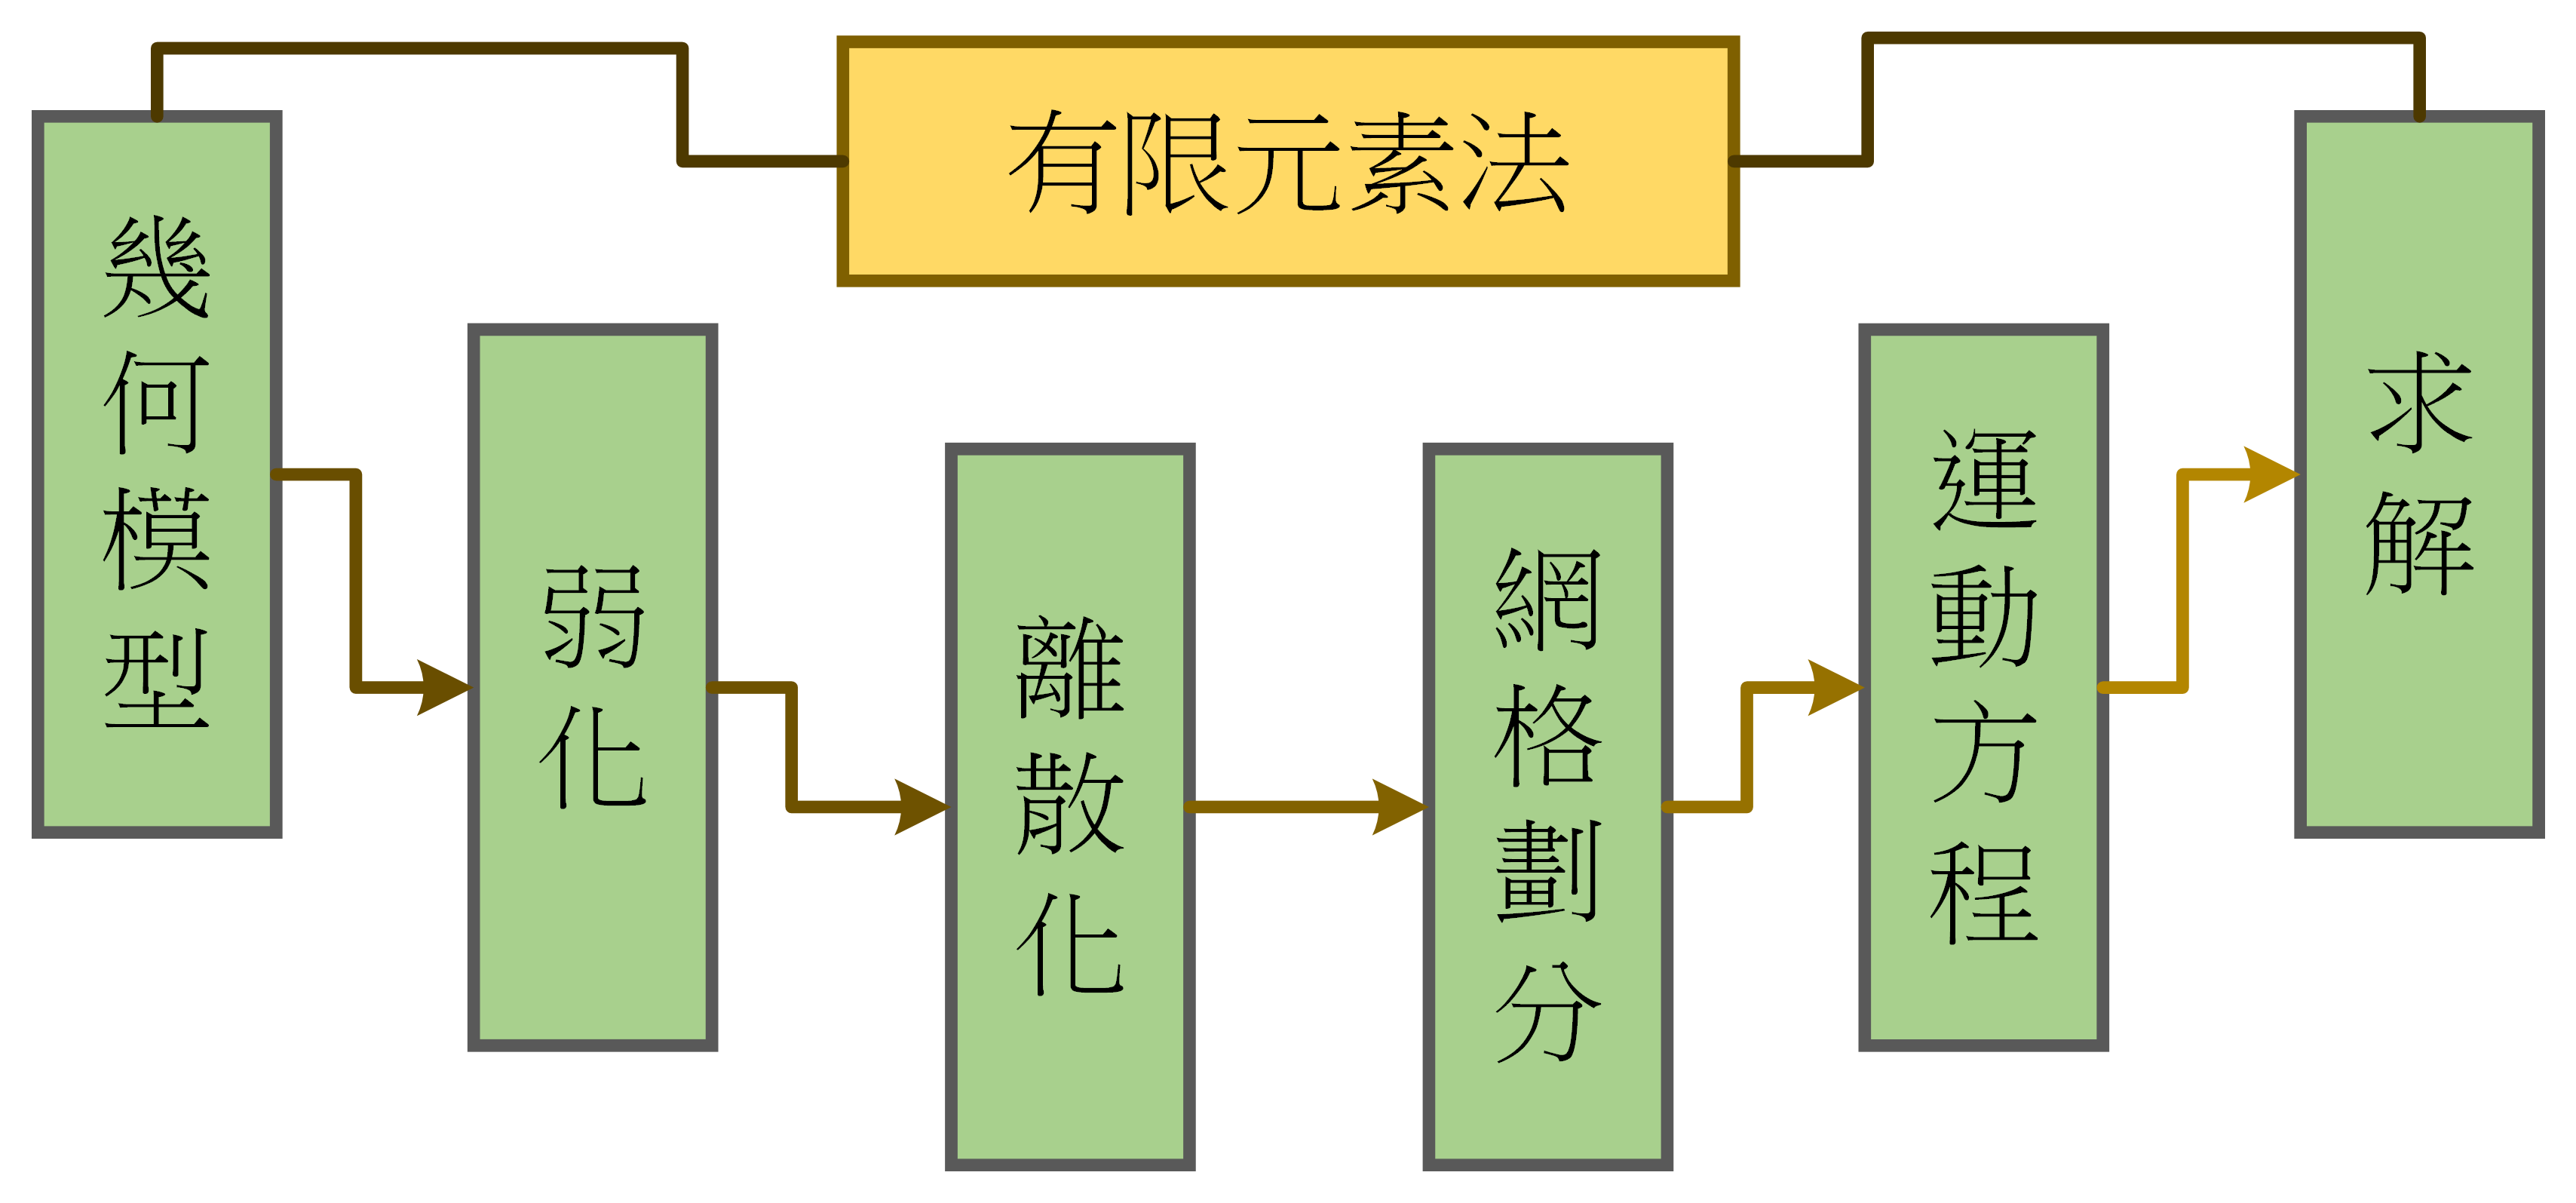
\includegraphics[width=13cm]{有限元素法分析流程}
\caption{\Large 有限元素法分析流程}\label{有限元素法分析流程}
\end{center}
\end{figure}

\begin{itemize}
\item 幾何模型:透過繪圖軟體將模型畫出,將模型以數據方式在電腦裡呈現二維或三維的外觀,便於軟體將其代入且計算。
\item 離散化及元素劃分:將物理系統或結構等連續變量通過計算轉換為數格元素的過程,對於複雜的連續變量,需先進行弱化的動作,才能進行離散化將其轉變為各個元素,此動作由分析軟體內部公式計算。
\item 導入函數並組成代數方程: 模型或問題不同,力學性質及物理方程相應的關係式(應力、應變、變形、熱傳等)也會跟著變化,因此需要根據對應的問題分別導入不同的函數,需在軟體內設定問題,讓其可以對特定問題進行求解,此動作為設計者提問,軟體負責計算。
\item 求解方程:在經過有限元素法分析後,將會在每個表面得知各元素的受力情況,設計者可以根據此數據了解到模型的受力狀態或位移及負載等相關訊息,以利於後續的設計或生產。
\end{itemize}
\newpage

\input{3_Quadruped_robot.tex}
\chapter{設計及模擬環境}
%\renewcommand{\baselinestretch}{10.0} %設定行距

%----------------設計環境---Solid Edge-----------------%
\section{設計環境---Solid Edge}
Solid Edge為一個由西門子PLM開發的三維特徵造型實體軟體,有著設計模型、模擬分析、製造及創成式設計等功能。\
設計者可以通過輸入參數以生成3D模型或是分析模型等動作,在2017年,Solid Edge也引進創成式設計功能,能夠依照多次疊代運算產生最終的優化結果。\\

本專題在模型參數上參考了許多設計者的機械狗模型,選擇了Solid Edge當作設計環境,因為其中包含了同步建模模型分析和創新式設計等功能,在原先參考的模型中繪製出類似的外觀,並對此建模進行尺寸調整,令設計更加的合理。\\

\begin{figure}[hbt!]
\center
\includegraphics[width=13cm]{model}
\caption{\Large 組合圖}
\label{model}
\end{figure}

\qquad 特徵建模
\begin{enumerate}
\item 順序建模:根據歷程記錄,可以返回到特徵建立過程的任何步驟,以編輯順序特徵。
\begin{figure}[hbt!]
\center
\includegraphics[width=13cm]{model}
\caption{\Large 組合圖}
\label{model}
\end{figure}

\item 同步建模:定義特徵形狀的面的集合,未保留同步特徵的建立方式歷程記錄。
\end{enumerate}
以下簡單介紹各功能:\\

\begin{figure}[hbt!]
\center
\includegraphics[width=13cm]{model}
\caption{\Large 組合圖}
\label{model}
\end{figure}

\begin{figure}[hbt!]
\center
\includegraphics[width=13cm]{model}
\caption{\Large 組合圖}
\label{model}
\end{figure}
%---------------路徑模擬-----Geogebra------------------%
\section{路徑模擬-----Geogebra}
誕生於2002年奧地利薩爾茨堡,其名稱由Geometry(幾何)和Algebra(代數)的混合詞,為一款動態幾何代數軟體,其特點為建立幾何物件,並保持其中連結關係,可以快速進行模擬計算並製作簡單動畫,作為教學演示軟體。\\

%---------------運動模擬-----CoppeliaSim------------------%
\section{運動模擬-----CoppeliaSim}
\qquad 使用原因
在此專題中,CoppeliaSim為我們提供了良好的模擬環境,透過帶入Solid Edge的模型,可以更加直觀的觀察到步行機構的運動軌跡,利用Python或是Lua程式,在開發環境趨近於現實的軟體中,有著相當大的自由度能對零件進行控制,每個轉軸、連桿、控制器等都可以在裡面設定,對尺寸及建模進行運動優化、調整提供了許多便利性,也節省多次修改實體模型的費用。\\

\qquad 常用功能
\qquad 以下為CoppeliaSim簡單介紹\

\begin{figure}[hbt!]
\center
\includegraphics[width=11cm]{CoppeliaSim}
\caption{\Large CoppeliaSim Logo}
\end{figure}
-------表格---------

\qquad RemoteAPI\\

RemoteAPI(Remote Application Programming Interface) 為CoppeliaSim API 框架之一,開發者可以使用自己熟悉的語言來編寫遠程通信的代碼,此框架允許應用程式在不同環境中通信及交互,使開發者可以訪問遠程計算資源及服務,實現分部式系統及協同處理、集成應用等功能。\\

-------表格---------
\newpage

%----------------程式控制--Python-----------------%
\section{程式控制--Python}
Python為創始人Guido van Rossum(吉多·范羅蘇姆)在1989年決心開發的指令解釋碼模式已成為ABC語言的繼承者,並打算用其替代Unix shell和C語言來進行系統管理。\\

為一開源並可擴充的語言,Python提供了豐富的API及工具,提供使用者能輕鬆使用的環境,其設計理念為<優雅><明確><簡單>\
在很多作業系統中,python被整合在其中為標準的系統元件,因此可在多個作業系統中運行,且能直接執行程式碼並即時查看成果,且在網路開發、數值分析、自動化測試等,其廣泛的應用領域和靈活性、不同環境中共享代碼,成為許多開發者及科學家的首選語言。\\

%------------------有限元素分析—Solid Edge---------------------%
\section{有限元素分析—Solid Edge}

關於有限元素分析,利用了Solid Edge作為我們的分析環境,選擇的原因在於模型是由Solid Edge建模的,繪製草圖完畢能夠直接對零件進行分析,不用在不同軟體中來回切換,透過新建的研究並定義材料或新增材質,設定負載位置,即可方便的對模型進行分析。\\

Solid Edge也能對零件直接進行創成式設計,即為在有限元素法分析過後,軟體經過多層的代數運算,在模型上新增或除料,對比之前工程師需要經過長久計算出可適用的模型,創成式設計大幅減少設計及時間成本,得益於近幾年電腦快速的發展,複雜的運算及設計通通可以透過創成式設計生成,不再受限於設計師的想法或經驗,並可以快速產生多個模型提供挑選。\\

%------------------有限元素分析—Ansys---------------------%
\section{有限元素分析—Solid Edge}

ANSYS Inc.成立於1970年,主要是工程模擬軟體和技術的研發,目的為減少設計周期及降低設計成本,在有限元分析、流體力學計算、設計優化等領域都有發展,有豐富的工具及靈敏度和擴展性,被工程師及設計師廣泛的使用\\

\newpage

\input{5_Quadruped_robot_Design_Kinematic_Simulation.tex}
\input{6_FEM_of_Quadruped_robot.tex}
\chapter{生成式設計}
運用電腦輔助系統的創造工具,利用軟體設計出所需的3D模型,輸入的參數或製作、預期要求,將成品利用電腦算法,強大的運算會模擬許多所有可能性及排列,並產生多個解決方案。\\

\begin{figure}[hbt!]
\center
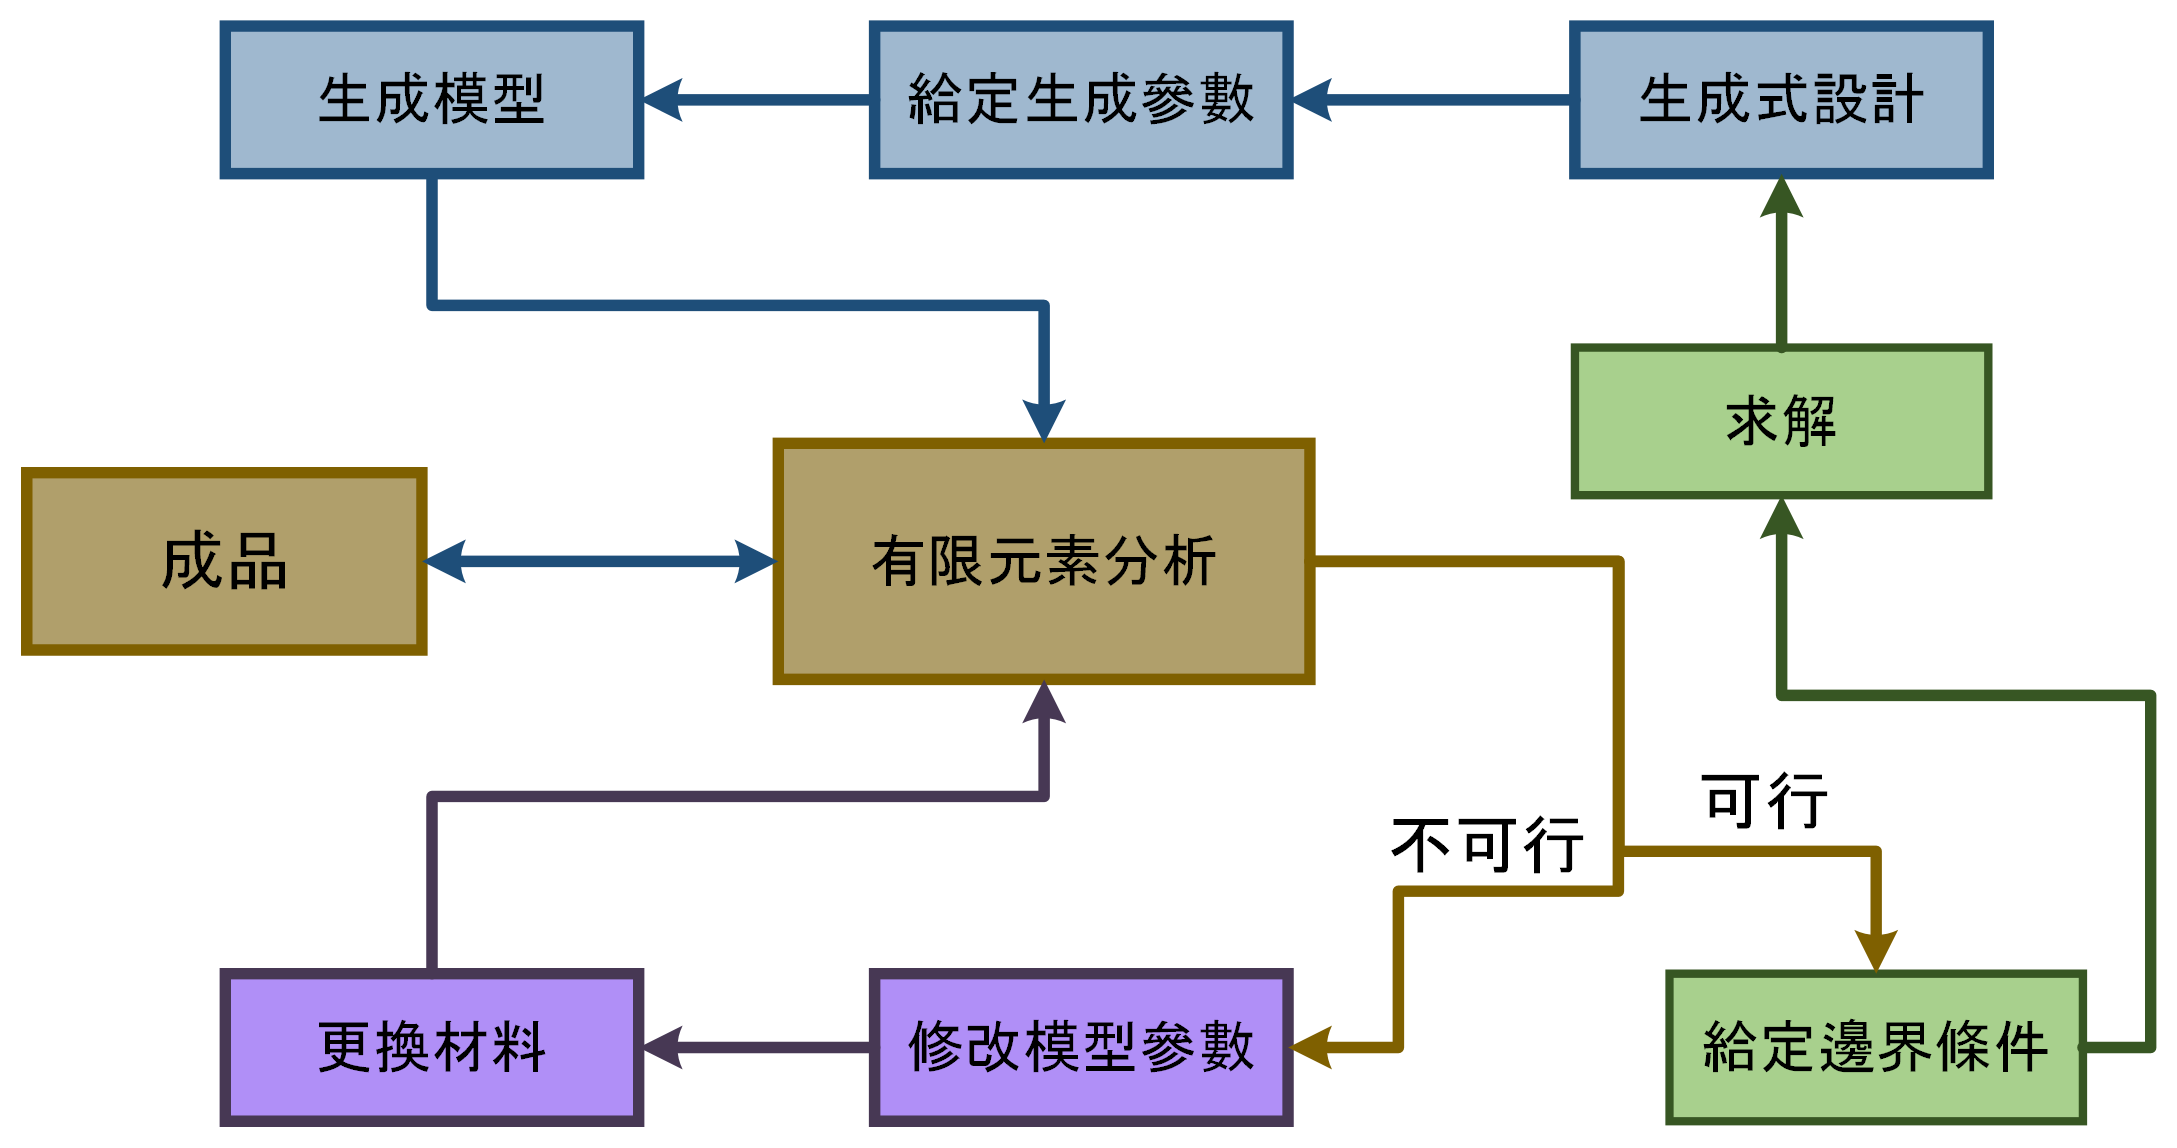
\includegraphics[width=10cm]{生成式流程}
\caption{\Large 生成式流程}
\label{生成式流程}
\end{figure}


主要依靠人工智能和機器學習來模仿自然界的進化設計方法,創造出許多種可能性,
利用AI運算生成整合並優化零件,創造出可能從未發現的幾何圖形,將產品創新優化,讓零件在輕盈的狀況下還保有堅韌程度,最大程度減低所需要耗費的人力、時間成本,讓成品可以快速並有效的產出。\\

%-----------------------生成式設計原理-------------------------%
\section{生成式設計原理}
生成式設計是一個迭代設計過程,透過軟體多次的分析與設計,生成符合製作條件的模型設計。生成式設計是一種電腦輔助設計的方法,利用軟體的AI智能算法,將設計者輸入的模型設計條件進行多次生成,並尋找出最佳設計。
生成式設計的主要功用為優化零件,不只能夠設計出更輕量化的零件,並且也能使各項性質提升,像是強度更強、更耐用、散熱快等。\\

%-----------------------設計流程-------------------------%
\section{設計流程}
\begin{itemize}
\item 確定設計目標:確定設計問題的範圍和目標
\item 新增條件約束:定義出用來生成設計方案的規則和條件,包括製造條件約束和幾何條件約束。
\item	執行生成:完成以上步驟,進行AI生成設計。
\item 優化生成結果:得到生成設計方案後,進行評估和優化,並對設計方案進行手動調整或修改,以便滿足特定的要求。\\

\end{itemize}

%-----------------------零件優化-------------------------%
\section{零件優化}
為了將零件輕量化,並維持其原本的零件強度,我們透過Solid Edge軟體將零件進行生成式設計,經過軟體的AI迭代算法以及多次修改設計參數,最後選擇最符合實際的設計。\

\begin{figure}[htbp]
  \centering
  \begin{minipage}{0.45\textwidth}
    \centering
    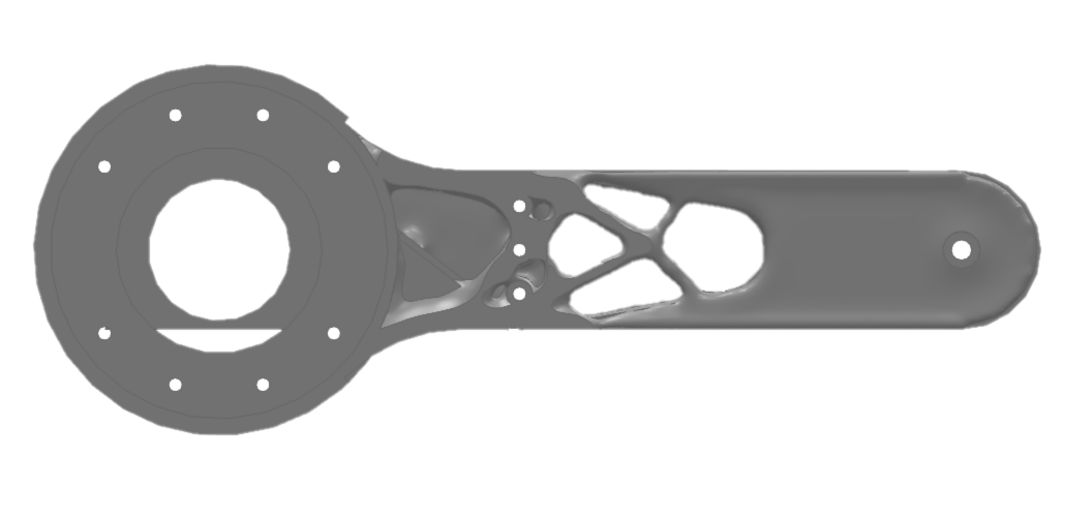
\includegraphics[width=\textwidth]{Leg1-1+1-5(拓樸)}
    \caption{Leg1-1+1-5(生成)}
    \label{Leg1-1+1-5(拓樸)}
  \end{minipage}
  \hfill
  \begin{minipage}{0.45\textwidth}
    \centering
    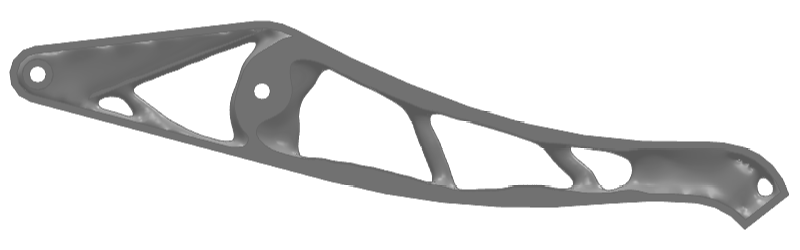
\includegraphics[width=\textwidth]{Leg4(拓樸)}
    \caption{Leg4(生成)}
    \label{Leg4(拓樸)}
  \end{minipage}
  \end{figure}

得到設計結果後,將原本的零件參考生成後的模型進行修改與挖空,這樣既保留所需的零件特徵,也達到了輕量化的目的,並使其外觀更加美觀。\

\begin{figure}[htbp]
  \centering
  \begin{minipage}{0.45\textwidth}
    \centering
    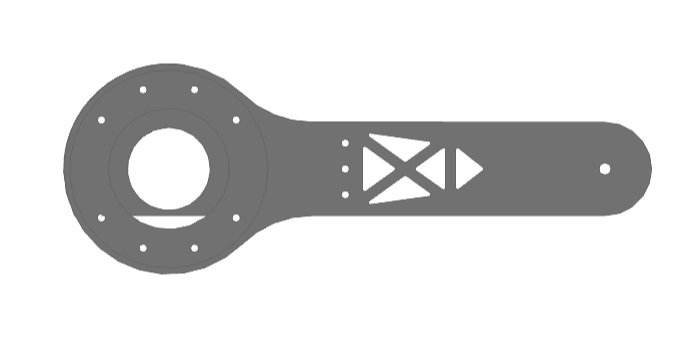
\includegraphics[width=\textwidth]{Leg1-1+1-5(輕量化)}
    \caption{Leg1-1+1-5(輕量化)}
    \label{Leg1-1+1-5(輕量化)}
  \end{minipage}
  \hfill
  \begin{minipage}{0.45\textwidth}
    \centering
    
\includegraphics[width=\textwidth]{Leg4(輕量化)}
    \caption{Leg4(輕量化)}
    \label{Leg4(輕量化)}
  \end{minipage}
  \end{figure}

將零件輕量化後,必須確認這樣的修改方式是否與初始零件的數值相同或更加強壯,因此我們將初始零件和輕量化零件進行分析比對,以查證輕量化方式是否有誤。\

\begin{figure}[hbt!]
\center
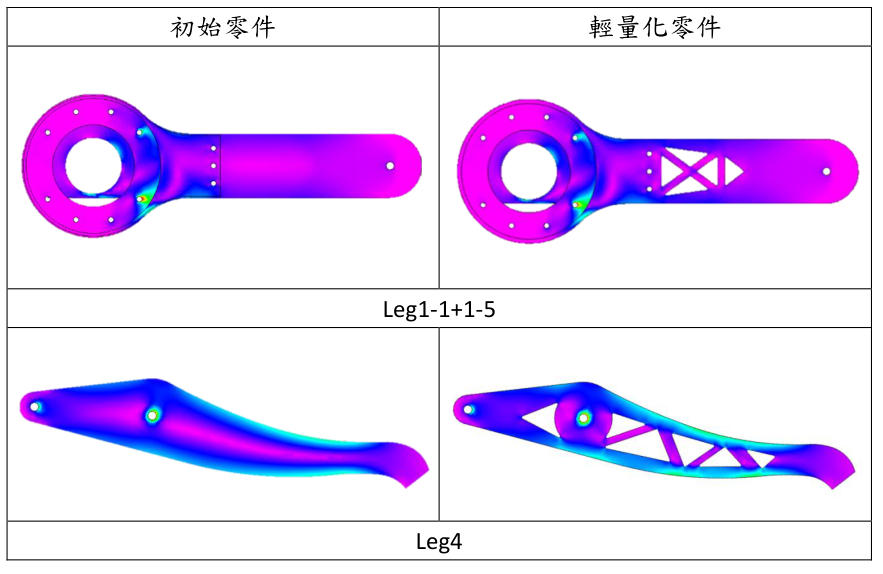
\includegraphics[width=16cm]{分析比對表(輕量化)}
\caption{\Large 分析比對表(輕量化)}
\label{分析比對表(輕量化)}
\end{figure}

\begin{table}[htb!]
  \center\large
  \caption{\Large leg1-1+1-5分析比對}
  \setlength{\tabcolsep}{1cm}{
  \begin{tabular}{|c|c|c|}
    \hline   
    &最大應力(MPa)& 最小安全係數  \\
    \hline 
    初始零件&69.4 & 0.937 \\
    \hline 
    輕量化零件 &69.9& 0.929 \\
    \hline
  \end{tabular}}
\end{table}

\begin{table}[htb!]
  \center\large
  \caption{\Large leg4分析比對}
  \setlength{\tabcolsep}{1cm}{
  \begin{tabular}{|c|c|c|}
    \hline   
    &最大應力(MPa)& 最小安全係數  \\
    \hline 
    初始零件&61.2 & 1.06 \\
    \hline 
    輕量化零件 &60& 1.08 \\
    \hline
  \end{tabular}}
\end{table}
\newpage

\chapter{總結}
本專題主要研究有限元素法的應用方式,探討了分析過程和應用方式,因為現實生活中不存在理想狀態下的剛體,每件物品、每個零件都是由柔性體所組合而成,隨著時間或外力的影響下會產生許多變量,而有限元素法則是以偏微分方程為基礎組成的分析法,主要用來對多種變量進行求解,以求出柔性體的受力狀況,有限元素法能對複雜模型分析的緣故,在近代被廣泛的應用在各種領域中,在建築或機械等地方都可以看見其身影。\\

四足機器人為一種模仿動物運動的機器人,可以幫助人類執行許多任務,而此設計中有著穩定性及負載的需求,所以步行裝置選用了四連桿為基礎架構,我們將四連桿機構帶入GeoGebra進行路徑分析,可以得到此機構的順逆向運動學,放入CoppeliaSim的擬真環境並運用了Python的作為控制程式,找到了最大的受力位置及角度。為了分析結果的準確性,我們帶入了兩種分析軟體進行比較,查看了分析結果並探討造成差異的原因,在之中發現了原先的ABS材料無法承受所預定的安全係數,因此在幾經尋找過後將全部零件材質換成了硬度較高的PLA,使四足機器人在日常做動時較不易損壞。\\

經過了上述的動作,我們已經驗證了5倍自身重量下步行機構依然可以正常做動,為了近一步增加其性能,我們將零件做生成式設計的步驟,對零件做輕量化處理且再次進行有限元素分析,卻保在四足機器人在減重後還保有一定強度。

\newpage

\chapter{未來展望}
\hspace{-1.7em} 軟體方面,此四足機器人的控制還可以更加深入得研究,對於控制元件的選用及電路的規劃,由於時間受限無法有著詳細介紹及實驗,要讓機器人可以實現在現實世界中,其中的問題還需要未來更為詳細得研究,有著計算單元、馬達控制、回饋單元、電池容量、效能平衡等,將其完善後加上目前的有限元分析,機器狗才能在現實中有著可預期並可控制的動作。\\

\hspace{-1.4em} 製成模板,以此專題分析為模板,將四足機器人各重要設計參數設定為可修改的,將一系列的設計道模擬再到分析製成一連串的程式,令後續使用者修改後就可以馬上進行分析,可以快速地透過模板生成可用的機器人。\\

\hspace{-1.4em} 模組化設計,將各部件例如步行機構或本體或電子元件等製成模組,使用者可以依照需求索取模組,可以對機器人進行修改,新增機械手臂或是捨棄步行機構換成履帶行走等,在經過設計者的開發有的多種可能性。\\

\newpage

%=---------------------參考文獻----------------------=%
\addcontentsline{toc}{chapter}{參考文獻} %新增目錄名稱
\newpage
\renewcommand\bibname{參~考~文~獻}
\begin{thebibliography}{99}  % 參考文獻印出之編號最寬為兩個字母寬
\bibitem 1\href{https://cn.comsol.com/multiphysics/fea-software?parent=finite-element-method-042-62-22}{https://cn.comsol.com/multiphysics/fea-software?parent=finite-element-method-042-62-22}
\bibitem 2\href{https://www.guyuehome.com/37628}{https://www.guyuehome.com/37628}
\bibitem 3\href{https://discord.com/channels/1056194150925615134/1056194150925615137/1113197208649609330}{https://discord.com/channels/1056194150925615134/1056194150925615137/1113197208649609330}
\bibitem 4\href{https://hdl.handle.net/11296/b8emug}{https://hdl.handle.net/11296/b8emug}
\bibitem 5\href{https://forums.autodesk.com/autodesk/attachments/autodesk/915/18197/2/一种四足步行机器人结构设计与分析.pdf}{https://forums.autodesk.com/autodesk/attachments/autodesk/915/18197/2/一种四足步行机器人结构设计与分析.pdf}
\bibitem 6\href{https://www.mdpi.com/2218-6581/12/1/28}{https://www.mdpi.com/2218-6581/12/1/28}
\bibitem 7\href{https://zh.wikipedia.org/zh-tw/有限元素法}{https://zh.wikipedia.org/zh-tw/有限元素法}
\bibitem 8\href{https://wiki.mbalib.com/zh-tw/有限单元法}{https://wiki.mbalib.com/zh-tw/有限单元法}
\bibitem 9\href{https://github.com/chaitravi-ce/Eklavya-QuadrupedMotionSimulation}{https://github.com/chaitravi-ce/Eklavya-QuadrupedMotionSimulation}
\bibitem 0\href{https://www.researchgate.net/publication/351078148_Design_and_Control_of_a_Open-Source_Low_Cost_3D_Printed_Dynamic_Quadruped_Robot}{https://www.researchgate.net/publication/351078148_Design_and_Control_of_a_Open-Source_Low_Cost_3D_Printed_Dynamic_Quadruped_Robot}\label{Quadruped_Robot}

%\bibitem 7\href
%\bibitem 8\href
%
%\bibitem 3\href{https://blog.csdn.net/Csdn_Darry/article/details/107142216}{https://blog.csdn.net/CsdnDarry/article/details/107142216}
\end{thebibliography}
\newpage

%=---------------附錄-----------------=%
\addcontentsline{toc}{chapter}{附錄} %新增目錄名稱
\begin{appendix}
\renewcommand{\thesection}{\bf 附錄 \Alph{section}}%設定標題名稱
\begin{center}
\fontsize{20pt}{0em}\selectfont\bf 附錄
\end{center}
\section*{LaTeX}
LaTex 為一種程式語言,支援標準庫 (Standard Libraries) 和外部程式庫 (External Libraries),不過與一般程式語言不同的是,它可以直接表述 Tex 排版結構,類似於 PHP 之於 HTML 的概念。但是直接撰寫 LaTex 仍較複雜,因此可以藉由 Markdown 這種輕量的標註式語言先行完成文章,再交由 LaTex 排版。
此專題報告採用編輯軟體為LaTeX,綜合對比Word編輯方法,LaTeX較為精準正確、更改、製作公式等,以便符合規範、製作。
 \begin{table}[htbp] %htbp代表表格浮動位置
			\centering%表格居中
			\caption{文字編輯軟體比較表}%表:標題
			\large%字體大小
			\label{tab_文字編輯軟體比較表:scale}
			\begin{tabular}{|c|c|c|c|c|c|c|}
			\hline
			\diagbox[width=5em]& 相容性 & 直觀性 & 文件排版 & 數學公式 & 微調細部\\ 
			\hline
			LaTeX 		&$\surd$&		&$\surd$&$\surd$&$\surd$\\
			\hline
			Word	 	&		&$\surd$&		&		&$\surd$\\
			\hline
			
			\end{tabular}
		\end{table}	
\end{appendix}
\begin{itemize} 
\item 特點:
\end{itemize}
\begin{enumerate}
\item 相容性:以Word為例會有版本差異,使用較高版本編輯的文件可能無法以較低的版本開啟,且不同作業系統也有些許差異;相比LaTeX可以利用不同編譯器進行編譯,且為免費軟體也可移植至可攜系統內,可以搭配Github協同編譯。
\item 文件排版:許多規範都會要求使用特定版型,使用文字編譯環境較能準確符合規定之版型,且能夠大範圍的自定義排定所需格式,並能不受之後更改而整體格式變形。
\item 數學公式呈現:LaTex可以直接利用本身多元的模組套件加入、編輯數學公式,在數學推導過程能夠快速的輸入自己需要的內容即可。
\item 細部調整:在大型論文、報告中有多項文字、圖片、表格,需要調整細部時,要在好幾頁中找尋,而LaTeX可以分段章節進行編譯,再進行合併處理大章節。
\end{enumerate}
\newpage

\section*{足端軌跡}
利用GeoGebra軟體求得各種足端軌跡所需的轉軸角度。\

\begin{figure}[htbp]
  \centering
  \begin{minipage}{0.45\linewidth}
    \centering
    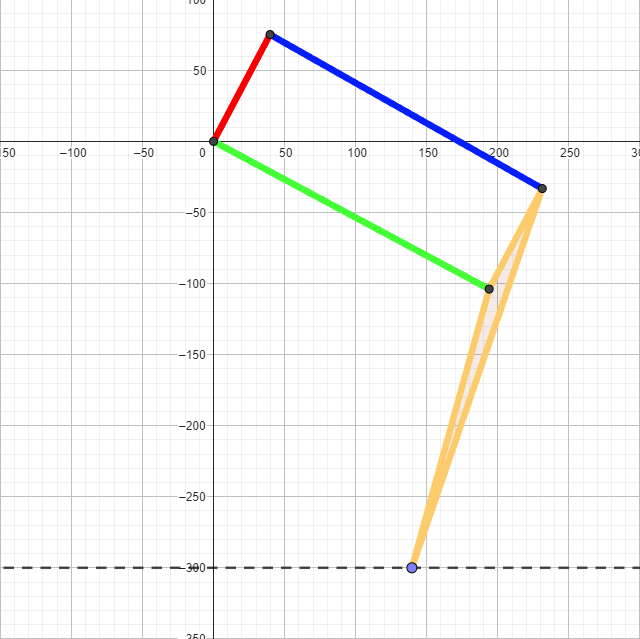
\includegraphics[height=5cm,width=5cm]{足端軌跡(直線)}
    \caption{足端軌跡(直線)}
    \label{足端軌跡(直線)}
  \end{minipage}
  \hfill
  \begin{minipage}{0.45\linewidth}
    \centering
    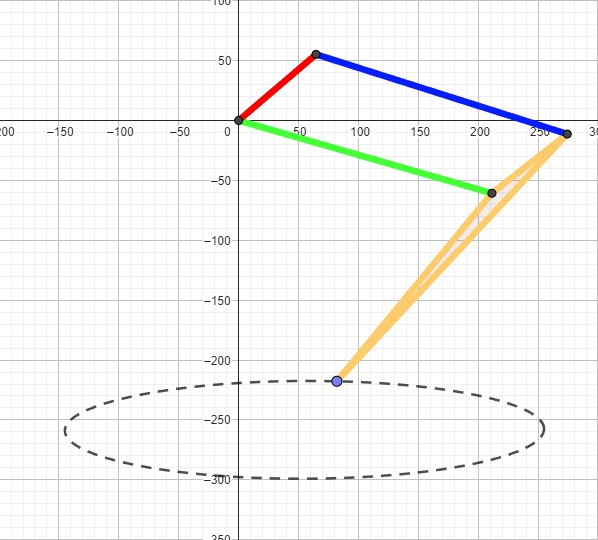
\includegraphics[height=5cm,width=5cm]{足端軌跡(橢圓)}
    \caption{足端軌跡(橢圓)}
    \label{足端軌跡(橢圓)}
  \end{minipage}
  
  \vspace{0.2cm} % 調整垂直間距
  
  \begin{minipage}{0.45\linewidth}
    \centering
    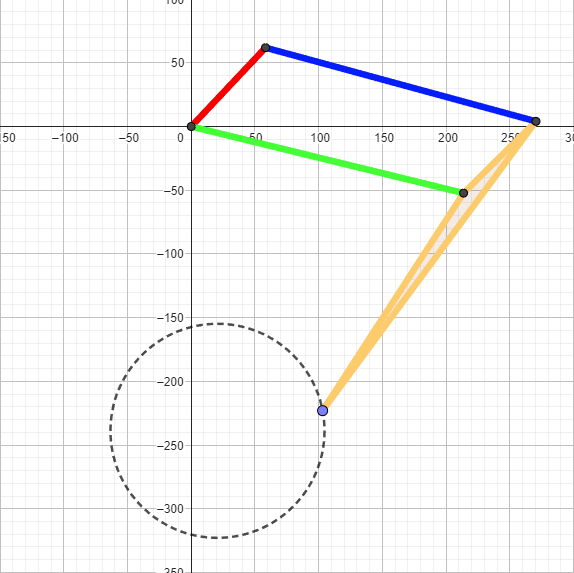
\includegraphics[height=5cm,width=5cm]{足端軌跡(圓形)}
    \caption{足端軌跡(圓形)}
    \label{足端軌跡(圓形)}
  \end{minipage}
  \hfill
  \begin{minipage}{0.45\textwidth}
    \centering
    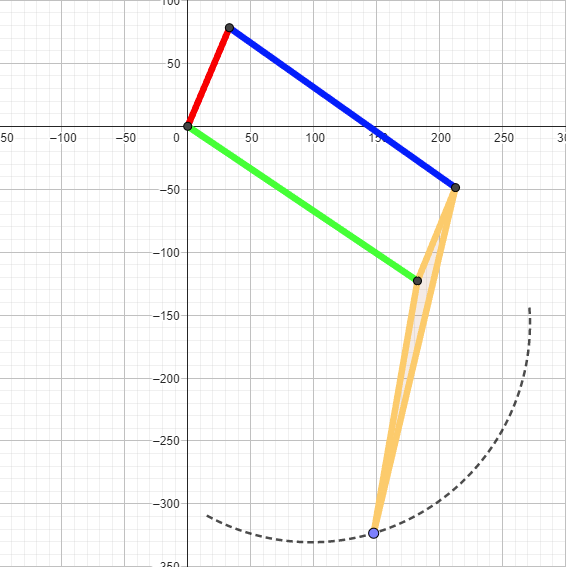
\includegraphics[height=5cm,width=5cm]{足端軌跡(弧線)}
    \caption{足端軌跡(弧線)}
    \label{足端軌跡(弧線)}
  \end{minipage}
  
  \vspace{0.2cm} % 調整垂直間距
  
  \begin{minipage}{0.45\linewidth}
    \centering
    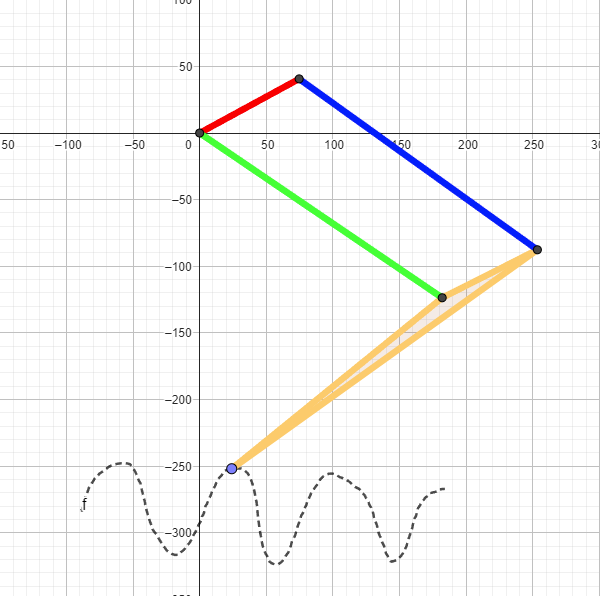
\includegraphics[height=5cm,width=5cm]{足端軌跡(不規則)}
    \caption{足端軌跡(不規則)}
    \label{足端軌跡(不規則)}
  \end{minipage}
\end{figure}
  
\newpage

\newpage
%=-------------作者簡介-----------------=%
    \addcontentsline{toc}{chapter}{作者簡介}
    \begin{center}
	\fontsize{20pt}{0em}\selectfont \bf{作者簡介}\\
	\end{center}	
	{\begin{textblock}{6}(0,0.5)
	\begin{figure}
	\includegraphics[width=1.25in]{40923231}
	\end{figure}
	\end{textblock}}
	{\renewcommand\baselinestretch{0.99}\selectfont %設定以下行距
	{\begin{textblock}{15}(3.5,0.7)%{寬度}(以左上角為原點之右移量,下移量)
	\noindent\fontsize{14pt}{0em}\selectfont \makebox[4em][s]{姓名}\enspace:\enspace
    \fontsize{14pt}{0em}\selectfont \makebox[4em][s]{楊子頡}\\     \hspace*{\fill} \\
    \fontsize{14pt}{0em}\selectfont \makebox[4em][s]{學號}\enspace:\enspace
    \fontsize{14pt}{0em}\selectfont \makebox[4em][s]{40923231} \\ %\makebox為文本盒子
    \hspace*{\fill} \\
    \fontsize{14pt}{0em}\selectfont \makebox[4em][s]{就讀學校}\enspace:\enspace
    \fontsize{14pt}{0em}\selectfont \makebox[9em][s]{國立虎尾科技大學}\\
    \fontsize{14pt}{0em}\selectfont \makebox[5em][s]{\quad}\enspace\enspace
    \fontsize{14pt}{0em}\selectfont \makebox[8em][s]{機械設計工程系}\\
    \hspace*{\fill} \\
    \fontsize{14pt}{0em}\selectfont \makebox[4em][s]{經歷}\enspace:\enspace
    \fontsize{14pt}{0em}\selectfont \makebox[9em][s]{國立彰化師範大學附屬高級工業職業學校}\\
    \fontsize{14pt}{0em}\selectfont \makebox[4em][s]{\quad}\enspace\enspace
    \fontsize{14pt}{0em}\selectfont \makebox[8em][s]{機電科}\\
    \end{textblock}}}
   % \hspace*{\fill} \\
   \vspace{2em}
	{\begin{textblock}{6}(0,2.3)
	\begin{figure}
	\includegraphics[width=1.15in]{40923233} 
    \end{figure}
    \end{textblock}}
    {\renewcommand\baselinestretch{0.99}
    \selectfont %設定以下行距
    {\begin{textblock}{15}(3.5,2.5) %{寬度}(以左上角為原點之右移量,下移量)
\noindent\fontsize{14pt}{0em}\selectfont \makebox[4em][s]{姓名}\enspace:\enspace
\fontsize{14pt}{0em}\selectfont \makebox[4em][s]{楊建霖}\\ 
\hspace*{\fill} \\
\fontsize{14pt}{0em}\selectfont \makebox[4em][s]{學號}\enspace:\enspace
\noindent\fontsize{14pt}{0em}\selectfont \makebox[4em][s]{40923233} \\ 
\hspace*{\fill} \\
\fontsize{14pt}{0em}\selectfont \makebox[4em][s]{就讀學校}\enspace:\enspace
\fontsize{14pt}{0em}\selectfont \makebox[9em][s]{國立虎尾科技大學}\\
\fontsize{14pt}{0em}\selectfont \makebox[5em][s]{\quad}\enspace\enspace
\fontsize{14pt}{0em}\selectfont \makebox[8em][s]{機械設計工程系}\\
\hspace*{\fill} \\
\fontsize{14pt}{0em}\selectfont \makebox[4em][s]{經歷}\enspace:\enspace
\fontsize{14pt}{0em}\selectfont \makebox[9em][s]{國立秀水高級工業職業學校}\\
\fontsize{14pt}{0em}\selectfont \makebox[4em][s]{\quad}\enspace\enspace
\fontsize{14pt}{0em}\selectfont \makebox[8em][s]{製圖科}\\
    \end{textblock}}}
    %\hspace*{\fill} \\
    \vspace{2em}
    {\begin{textblock}{6}(0,4.1)
    \begin{figure}
        \includegraphics[width=1.15in]{40923235} %{}內是圖片文件的相對路徑
    \end{figure}
    \end{textblock}}
    {\renewcommand\baselinestretch{0.99}\selectfont %設定以下行距
    {\begin{textblock}{15}(3.5,4.3) %{寬度}(以左上角為原點之右移量,下移量)
\noindent\fontsize{14pt}{0em}\selectfont \makebox[4em][s]{姓名}\enspace:\enspace%\noindent指定首行不進行縮排
\fontsize{14pt}{0em}\selectfont \makebox[4em][s]{詹侑儒}\\ 
\hspace*{\fill} \\
\noindent\fontsize{14pt}{0em}\selectfont \makebox[4em][s]{學號}\enspace:\enspace
\noindent\fontsize{14pt}{0em}\selectfont \makebox[4em][s]{40923235} \\ %\makebox為文本盒子
\hspace*{\fill} \\
\noindent\fontsize{14pt}{0em}\selectfont \makebox[4em][s]{就讀學校}\enspace:\enspace
\noindent\fontsize{14pt}{0em}\selectfont \makebox[9em][s]{國立虎尾科技大學}\\
\noindent\fontsize{14pt}{0em}\selectfont \makebox[5em][s]{\quad}\enspace\enspace
\noindent\fontsize{14pt}{0em}\selectfont \makebox[8em][s]{機械設計工程系}\\
\hspace*{\fill} \\
\noindent\fontsize{14pt}{0em}\selectfont \makebox[4em][s]{經歷}\enspace:\enspace
\fontsize{14pt}{0em}\selectfont \makebox[9em][s]{新北市立新莊高級中學}\\
    \end{textblock}}}
   % \hspace*{\fill} \\
   \vspace{2em}
    {\begin{textblock}{6}(0,5.9)
    \begin{figure}
        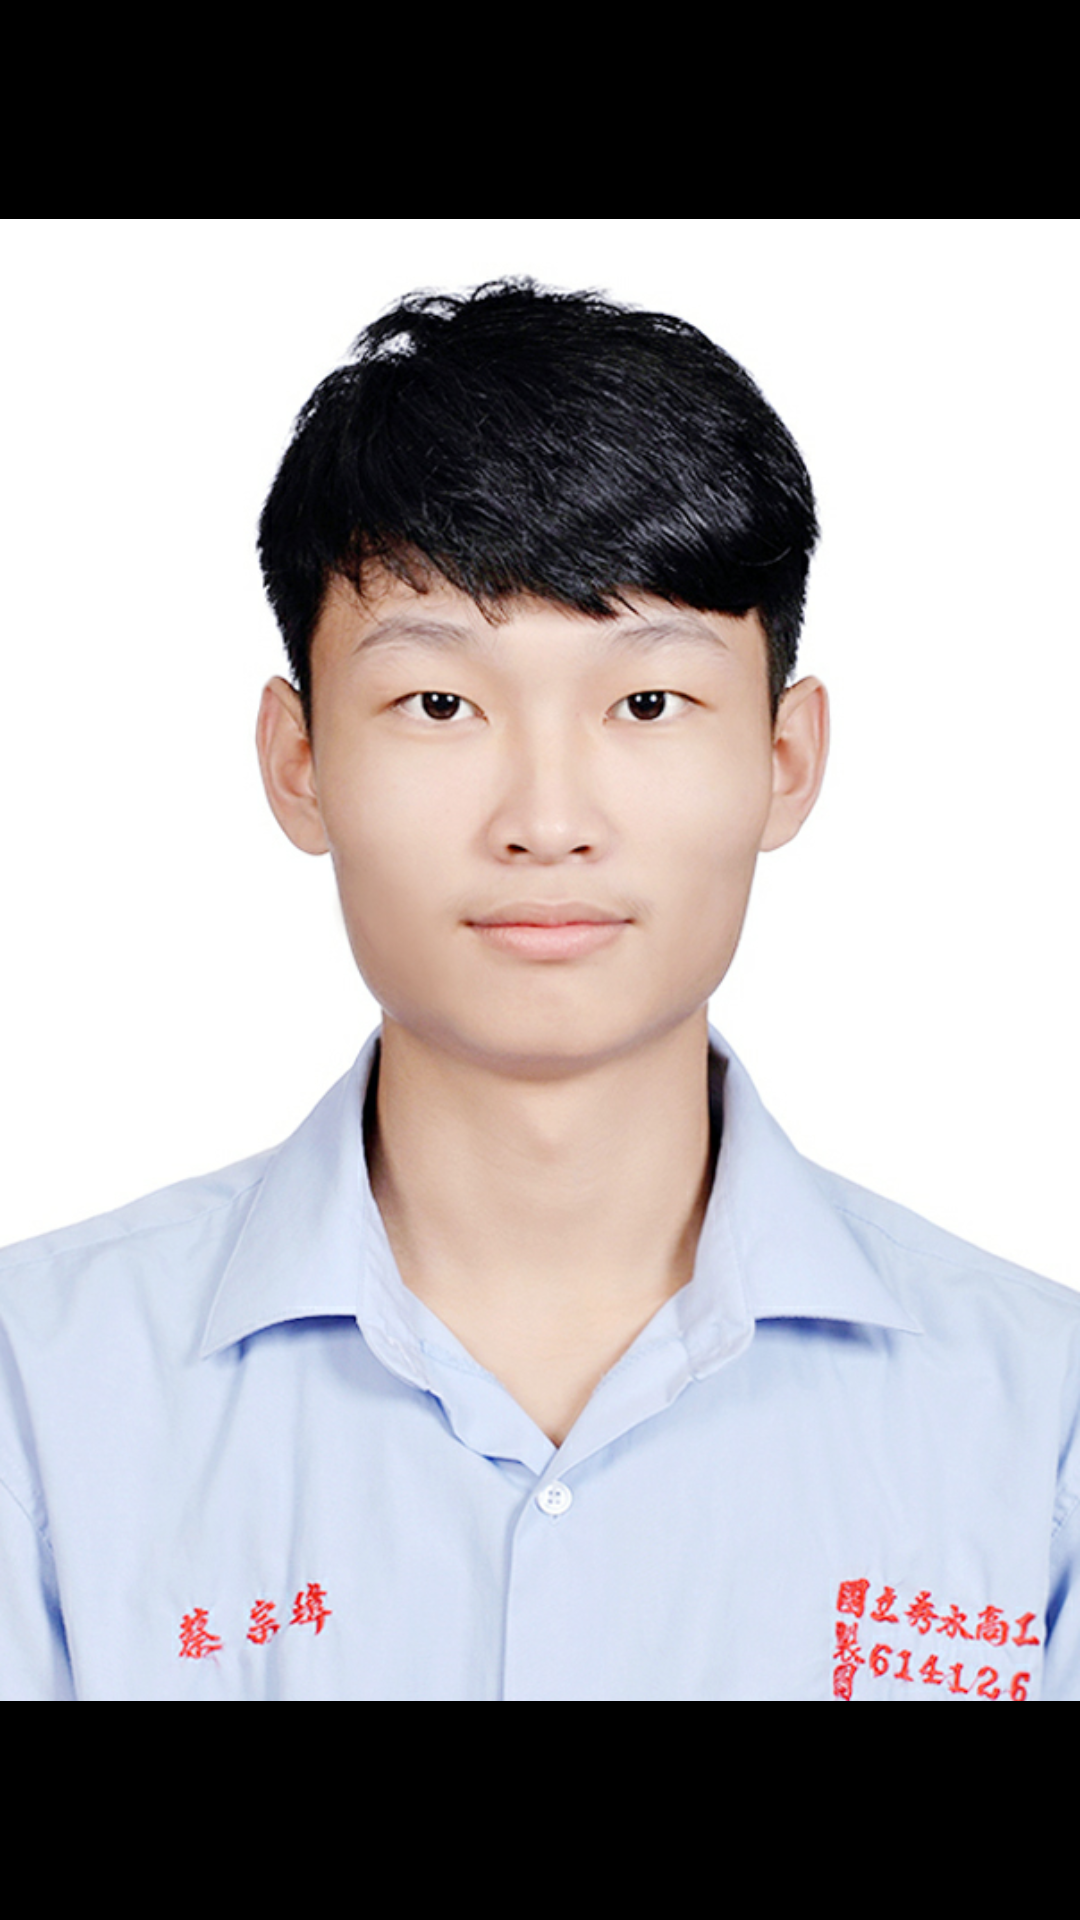
\includegraphics[width=1.15in]{40923240} %{}內是圖片文件的相對路徑
    \end{figure}
    \end{textblock}}
    {\renewcommand\baselinestretch{0.99}\selectfont %設定以下行距
    {\begin{textblock}{15}(3.5,6.1) %{寬度}(以左上角為原點之右移量,下移量)
\noindent\noindent\fontsize{14pt}{0em}\selectfont \makebox[4em][s]{姓名}\enspace:\enspace
\noindent\fontsize{14pt}{0em}\selectfont \makebox[4em][s]{蔡宗瑋}\\ \hspace*{\fill} \\
\noindent\fontsize{14pt}{0em}\selectfont \makebox[4em][s]{學號}\enspace:\enspace
\noindent\fontsize{14pt}{0em}\selectfont \makebox[4em][s]{40923240} \\ \hspace*{\fill} \\
\noindent\fontsize{14pt}{0em}\selectfont \makebox[4em][s]{就讀學校}\enspace:\enspace
\noindent\fontsize{14pt}{0em}\selectfont \makebox[9em][s]{國立虎尾科技大學}\\
\noindent\fontsize{14pt}{0em}\selectfont \makebox[5em][s]{\quad}\enspace\enspace
\noindent\fontsize{14pt}{0em}\selectfont \makebox[8em][s]{機械設計工程系}\\
\hspace*{\fill} \\
\noindent\fontsize{14pt}{0em}\selectfont \makebox[4em][s]{經歷}\enspace:\enspace
\fontsize{14pt}{0em}\selectfont \makebox[9em][s]{國立秀水高級工業職業學校}\\
\fontsize{14pt}{0em}\selectfont \makebox[4em][s]{\quad}\enspace\enspace
\fontsize{14pt}{0em}\selectfont \makebox[8em][s]{製圖科}\\
    \end{textblock}}}
\newpage

%=----------------書背----------------------=%
\pagestyle{empty}%設定沒有頁眉和頁腳
\begin{center}
\fontsize{0.001pt}{1pt}\selectfont .\\
\vspace{4em}
\fontsize{30pt}{30pt}\selectfont 【05】 \\
\fontsize{20pt}{20pt}\selectfont
\vspace{0.5em}
分\\
類\\
編\\
號\\
\vspace{0.5em}
\hspace{-0.5em}:\\
\vspace{0.5em}
\rotatebox[origin=cc]{270}{\sectionef\LARGE \textbf{112-4-CAE-3006、3004}}\\ %旋轉
\vspace{0.5em}
有\\
限\\
元\\
素\\
法\\
在\\
四\\
足\\
機\\
器\\
人\\
上\\
的\\
應\\
用\\
\vspace{1.5em}
一\\
\vspace{0.5em}
百\\
\vspace{0.5em}
一\\
\vspace{0.5em}
十\\
\vspace{0.5em}
三\\
\vspace{0.5em}
級\\

\end{center}
%\newpage
%\begin{landscape}  %橫式環境
%\begin{center}
%\fontsize{0.001pt}{1pt}\selectfont .
%\vspace{70mm}
%\rotatebox[origin=cc]{90}{\LARGE 【14】}\rotatebox[origin=cc]%{180}{\LARGE 1-2-APP-8765} %旋轉
%\end{center}
%\end{landscape}
\end{document}
